\documentclass[techmemo]{ecmwfrep}%
\usepackage{graphicx}
\usepackage{array}
\usepackage{natbib}

%%%%%%%%%%%%%%%%%%%%%%%%%%%%%%%%%%%%%%%%%%%%%%%%%%%%%%%%%%%%%%%%%%%%%%%%%%%%
\title{ecPoint-Calibrate: more than an off-the-shelf number cruncher to grow decision trees}
\headertitle{ecPoint-Calibrate} 
\coverauthor{Fatima M. Pillosu, Daniel Tipping, Tim Hewson \\(Forecasts Department)}
\seriesnumber{909}
\date{September 2023}
%%%%%%%%%%%%%%%%%%%%%%%%%%%%%%%%%%%%%%%%%%%%%%%%%%%%%%%%%%%%%%%%%%%%%%%%%%%%

\begin{document}
\maketitle
\begin{abstract}
Lorem ipsum dolor sit amet, consectetur adipiscing elit. Morbi elementum orci nec mauris mollis ornare. Pellentesque congue purus sapien, vitae sagittis massa auctor sed. Pellentesque gravida sem eget orci dapibus interdum. Suspendisse vitae libero ut tortor fermentum egestas. Nullam lacinia ultricies dapibus. Nam vitae porttitor turpis, eu hendrerit lectus. Nulla sollicitudin velit et elit porta eleifend. Praesent laoreet eros vitae nibh tempor, bibendum lacinia ante rhoncus. Pellentesque consequat in diam non porta. Nunc sollicitudin purus et molestie suscipit. Curabitur aliquam ipsum vel ligula facilisis ullamcorper. Donec sollicitudin sapien in dui lobortis, et efficitur tortor dictum. Nullam eu semper elit, a lacinia nulla. Cras nec interdum arcu. Sed non scelerisque urna, non viverra ante. Cras elementum justo ut mi porttitor fringilla sit amet sed mauris. Vestibulum ac ex venenatis, malesuada quam venenatis, semper ipsum. Cras ac lorem quis nisi porta pharetra ut venenatis erat. Curabitur a aliquet metus. Phasellus vitae lectus.
\end{abstract}

%%%%%%%%%%%%%%%%%%%%%%%%%%%%%%%%%%%%%%%%%%%%%%%%%%%%%%%%%%%%%%%%%%%%%%%%%
\section*{Plain language summary}
Lorem ipsum dolor sit amet, consectetur adipiscing elit. Morbi elementum orci nec mauris mollis ornare. Pellentesque congue purus sapien, vitae sagittis massa auctor sed. Pellentesque gravida sem eget orci dapibus interdum. Suspendisse vitae libero ut tortor fermentum egestas. Nullam lacinia ultricies dapibus. Nam vitae porttitor turpis, eu hendrerit lectus. Nulla sollicitudin velit et elit porta eleifend. Praesent laoreet eros vitae nibh tempor, bibendum lacinia ante rhoncus. Pellentesque consequat in diam non porta. Nunc sollicitudin purus et molestie suscipit. Curabitur aliquam ipsum vel ligula facilisis ullamcorper. Donec sollicitudin sapien in dui lobortis, et efficitur tortor dictum. Nullam eu semper elit, a lacinia nulla. Cras nec interdum arcu. Sed non scelerisque urna, non viverra ante. Cras elementum justo ut mi porttitor fringilla sit amet sed mauris. Vestibulum ac ex venenatis, malesuada quam venenatis, semper ipsum. Cras ac lorem quis nisi porta pharetra ut venenatis erat. Curabitur a aliquet metus. Phasellus vitae lectus.

%%%%%%%%%%%%%%%%%%%%%%%%%%%%%%%%%%%%%%%%%%%%%%%%%%%%%%%%%%%%%%%%%%%%%%%%%
\section*{List of abbreviations}

\begin{tabular}{r l}
\hline
ABBREVIATION & DESCRIPTION \\
\hline
BP & Break point \\
CVP & Conditional verification plot \\
DT & Decision tree \\
ECMWF & European centre for medium-range weather forecasts \\
ENS & ECMWF ensemble forecasts \\
FE & Forecast error \\
FER & Forecast error ratio \\
G-WT & Grid-box weather type \\
GUI & Graphical user interface \\
K-S test & Kolmogorov-Smirnov test \\
MF & Mapping function \\
NWP & Numerical weather prediction \\
PDT & Point data table \\
RC & Remote calibration \\
\end{tabular}

%%%%%%%%%%%%%%%%%%%%%%%%%%%%%%%%%%%%%%%%%%%%%%%%%%%%%%%%%%%%%%%%%%%%%%%%%
\section{Introduction}

While numerical weather prediction (NWP) model outputs continue to improve \citep{Bauer2015, Bauer2021}, they remain susceptible to biases \citep{Lavers2021} and representative errors \citep{Haiden2018}. Statistical post-processing can downscale raw NWP model outputs to satisfy users’ demands for local predictions while also enhancing reliability and skill \citep{Wilks2019}. Since 2016, the European Centre for Medium-range Weather Forecasts (ECMWF) has been developing ecPoint, a statistical post-processing technique to anticipate sub-grid variability and improve biases in their ensemble (ENS) forecasting system \citep{Hewson2021}. This article provides an overview of ecPoint-Calibrate, the calibration software at the heart of ecPoint (see Figure \label{Main_Menu} \ref{Main_Menu}).

As advocated by \cite{Hemri2014}, statistical corrections of NWP model outputs are today considered integral to operational forecasting systems, regardless of how sophisticated the model is, since end users still benefit from improvements imparted by post-processing. For a comprehensive review of state-of-the-art statistical post-processing techniques, see \cite{Vannitsem2021}. When numerical post-processed NWP model outputs are unavailable, forecasters often rely on heuristic methods to enhance raw model predictions for specific locations \citep{Doswell2004}. Unlike the objective methods reviewed by \cite{Vannitsem2021}, \cite{Doswell2004} refers to heuristics as a general term for the subjective methods humans use for making judgments in the presence of uncertainty. Although heuristics can suffer from forecasters’ adaptation lags to new model versions and forecasters’ inherent knowledge biases, reliable and skilful predictions for specific locations can be issued using this post-processing approach \citep{Hoffman2017}. In ecPoint-Calibrate, forecasters’ heuristics are put to the test and complemented by the precision and consistency of objective algorithms.

Since decision trees (DTs) are considered one of the best tools for knowledge discovery and inductive rule-building \citep{Murthy1998, Rokach2014, Kotsiantis2013, Loh2014, Chase2022, Costa2023}, ecPoint-Calibrate employs a DT algorithm to incapsulate forecasters’ heuristics. DTs have stood the test of time since they originally appeared in the 1960s \citep{Morgan1963} due to their simplicity (e.g., they require little data preparation, work very well with simple tabular data, and are not computationally expensive to run), robustness (e.g., they are not heavily affected by missing values or outliers), and interpretability (e.g., model’s decisions can be easily understood and visualised even for large datasets). DTs have recently attracted more attention alongside other machine learning systems such as neural networks and deep learning \citep{Chase2023} due to the rising interest in explainable machine learning, i.e., models that can be understood by humans \citep{Rudin2019,Roscher2020}. While DTs can be vulnerable to overfitting, algorithms like “random forest” can counter this \citep{Abdulkareem2021}. However, this algorithm will be less interpretable than individual decision trees, the prediction creation process might be slow, and the model size can be fairly large, making it inefficient for real-time applications. ecPoint-Calibrate is built using a deterministic DT algorithm, emphasising the developers commitment to simplicity and clarity.

While DTs are provided with five-star software support (e.g., ScikitLearn, XGBoost, CatBoost), ecPoint-Calibrate uses a semi-automatic DT algorithm to allow expert elicitation (e.g., from forecasters, NWP developers, and verification experts) guide the final shape of the DT. Expert elicitation draws upon the knowledge and insights of experts to summarise, interpret, and reduce the dimensionality of complex data \citep{OHagan2019}. Expert elicitation should nonetheless be used judiciously, considering its subjectivity \citep{Morgan2014}. A combined approach, using both expert judgment and quantitative analysis, can offer the most comprehensive and accurate understanding of the data. For example, ecPoint-Calibrate builds the DTs using expert elicitation to define the list of predictors to analyse but then uses the Kolmogorov-Smirnov test (K-S test) to help define the most appropriate break points (BP) in the DT.

Originating as a set of Matlab scripts boasting high performance, flexibility, and careful error management, ecPoint-Calibrate evolved into a graphical user interface (GUI) within the project “ECMWF Summer of Weather Code” to better meet user needs. While retaining computational high performance, the GUI followed best practices  to improve user-friendliness, e.g., the GUI is more intuitive and easier to interact with than the old command-line interface, efficiency, e.g., the GUI streamlines the calibration workflow, and error minimisation, e.g., the GUI offers predefined options, integrated help options, and error messages \citep{Preece1994}. The GUI also introduced two main novel features. It offers the full customisation and visualisation of the DTs, facilitating the introduction of physical reasoning during the DT creation phase. It also includes the option to display conditional verification map plots to inform the operator about data behaviours.

ecPoint-Calibrate has been successfully used at ECMWF in the operational calibration of 12-hourly rainfall forecasts \citep{Hewson2019}. Furthermore, the projects MISTRAL and HIGHLANDER have leveraged it for the calibration of the 6-hourly rainfall forecasts \citep{Gascón2023} and the extended-range and ERA5 24-hourly rainfall and temperature \citep{Hewson2023}.

The remainder of the paper is structured as follows. Section 2 briefly describes the software architecture. Section 3 explains some foundational concepts of the calibration methodology. Sections 4, 5, and 6 describe the calibration approach, workflow, and main outputs. Section 7 presents examples of downstream use cases. The paper is concluded with a summary section.

\begin{figure}
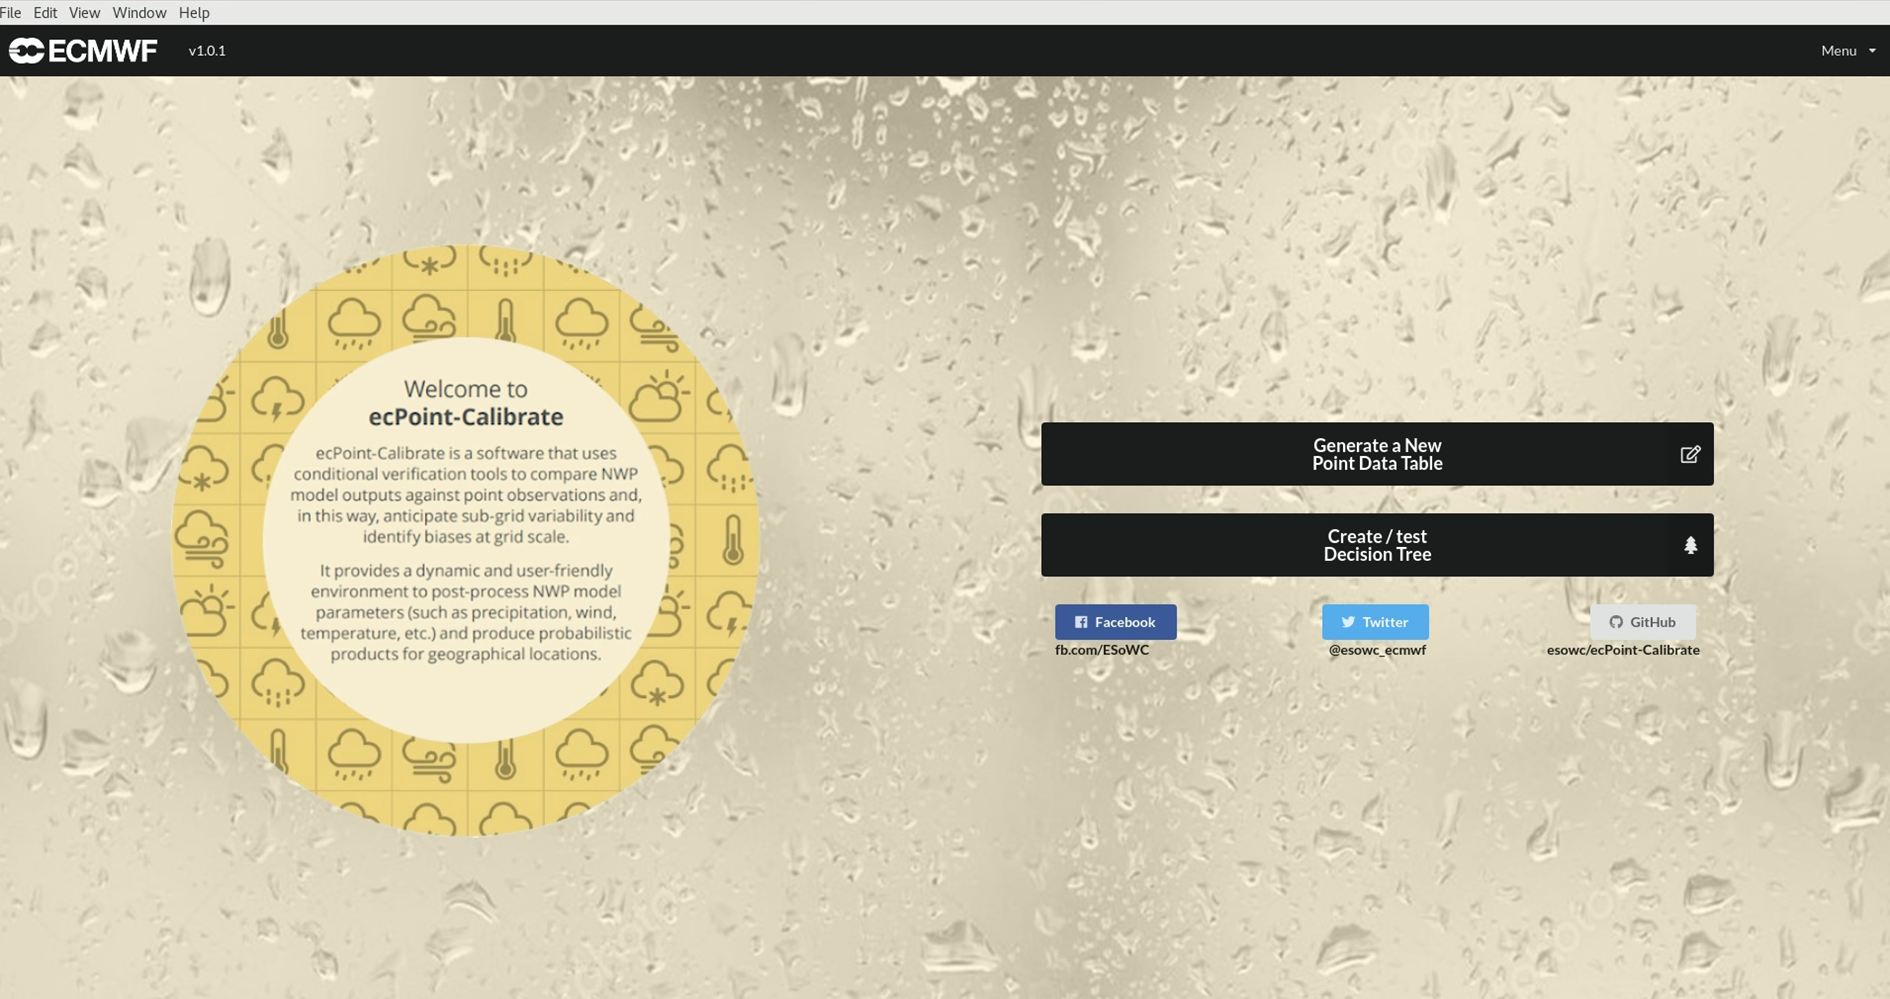
\includegraphics{Figures/Main_Menu.png}
\caption{Screenshot of ecPoint-Calibrate's main menu.}
\label{Main_Menu}
\end{figure}

%%%%%%%%%%%%%%%%%%%%%%%%%%%%%%%%%%%%%%%%%%%%%%%%%%%%%%%%%%%%%%%%%%%%%%%%%
\section{Software architecture, 200 words}
Lorem ipsum dolor sit amet, consectetur adipiscing elit. Proin vestibulum tincidunt leo. Proin vitae lorem non purus vehicula feugiat. Curabitur quis consectetur nisl. Proin lobortis dictum congue. Nullam sed mattis quam. Nullam sit amet lacus turpis. Ut sed nunc eu nisl varius tristique. Ut fermentum pharetra leo, eget vehicula metus gravida quis. Proin sodales lacus risus, sed iaculis nisi luctus at. Nulla fringilla dapibus tortor, in blandit justo blandit at. Quisque sit amet leo nisl. Donec tempus orci enim, eu porttitor lacus porta nec. Orci varius natoque penatibus et magnis dis parturient montes, nascetur ridiculus mus. Nam a purus sagittis, sollicitudin libero sit amet, commodo arcu. Aliquam erat volutpat. Aenean ut est porttitor, lobortis dui at, facilisis sapien. Proin dapibus leo in blandit posuere. Fusce fringilla sem mattis sapien euismod, eget imperdiet enim vehicula. Suspendisse sem sapien, congue at sapien at, pretium vehicula purus. Vestibulum sed suscipit mauris. Ut id elit ligula. Maecenas a fermentum dolor, quis gravida lorem. Nam convallis pharetra purus. Mauris sapien eros, ultricies quis felis at, interdum mattis augue. Nullam iaculis suscipit condimentum. Curabitur libero sapien, porttitor eu sapien a, elementum hendrerit tellus. Duis arcu nibh, feugiat ut mi in, finibus sodales dui. Curabitur vehicula lorem.. Vestibulum molestie pretium ultrices. Nunc finibus condimentum lectus sit amet tincidunt. Vivamus dignissim ex eget pretium egestas.

%%%%%%%%%%%%%%%%%%%%%%%%%%%%%%%%%%%%%%%%%%%%%%%%%%%%%%%%%%%%%%%%%%%%%%%%%
\section{Software philosophy}

\subsection{Remote calibration (200 words)}

Post-processing methods must be calibrated. For this purpose, post-processing methods compare forecast parameters with observations. The majority of the post-processing methods are typically applied to specific locations (references). This means that, to create a timeseries that contains most of the types of rainfall event that can affect the location of interest, a time series of at least 20-years is required to produce robust statistics (reference). 

In the ecPoint post-processing technique, it is assumed that the relationships between forecasts and observations are independent of geographical location, except for those cases where geographical representations are indirect represented within certain predictor classes that consider topographic sub-grid complexity, population density, local solar time, etc. This assumption, named within the ecPoint technique, "remote calibration" is a re-iteration of the universality of physical laws, and recognises that latitude-longitude coordinates should not, of themselves, determine any forecasts-observation relationships. This is a key difference between the ecPoint method and other post-processing methods, such as EMOS, where location is everything. Whilst most recent studies have successfully relaxed this constraint via data pooling, wherein observations from sites that are geographically close and that have a similar topographical aspect are grouped together for calibration (reference), ecPoint goes much further by pooling in a highly dynamic way according to governing variable ranges, without geographical constraints being imposed from the outset. Figure ... shows the location of points informing the post-processing of the category of "heavy rain" in the UK. This is an extremely powerful innovation because it allows the size of the calibration dataset to be increased by several orders of magnitude compared to classic post-processing techniques. The "remote calibration" approach is indeed key to to being able to generate many complex yet complete mapping functions using as little as one year of calibration data, without having to be too concerned about overfitting (the leaves of the DT tend to be constructed with at least 1000 or more data points).
 
\begin{figure}
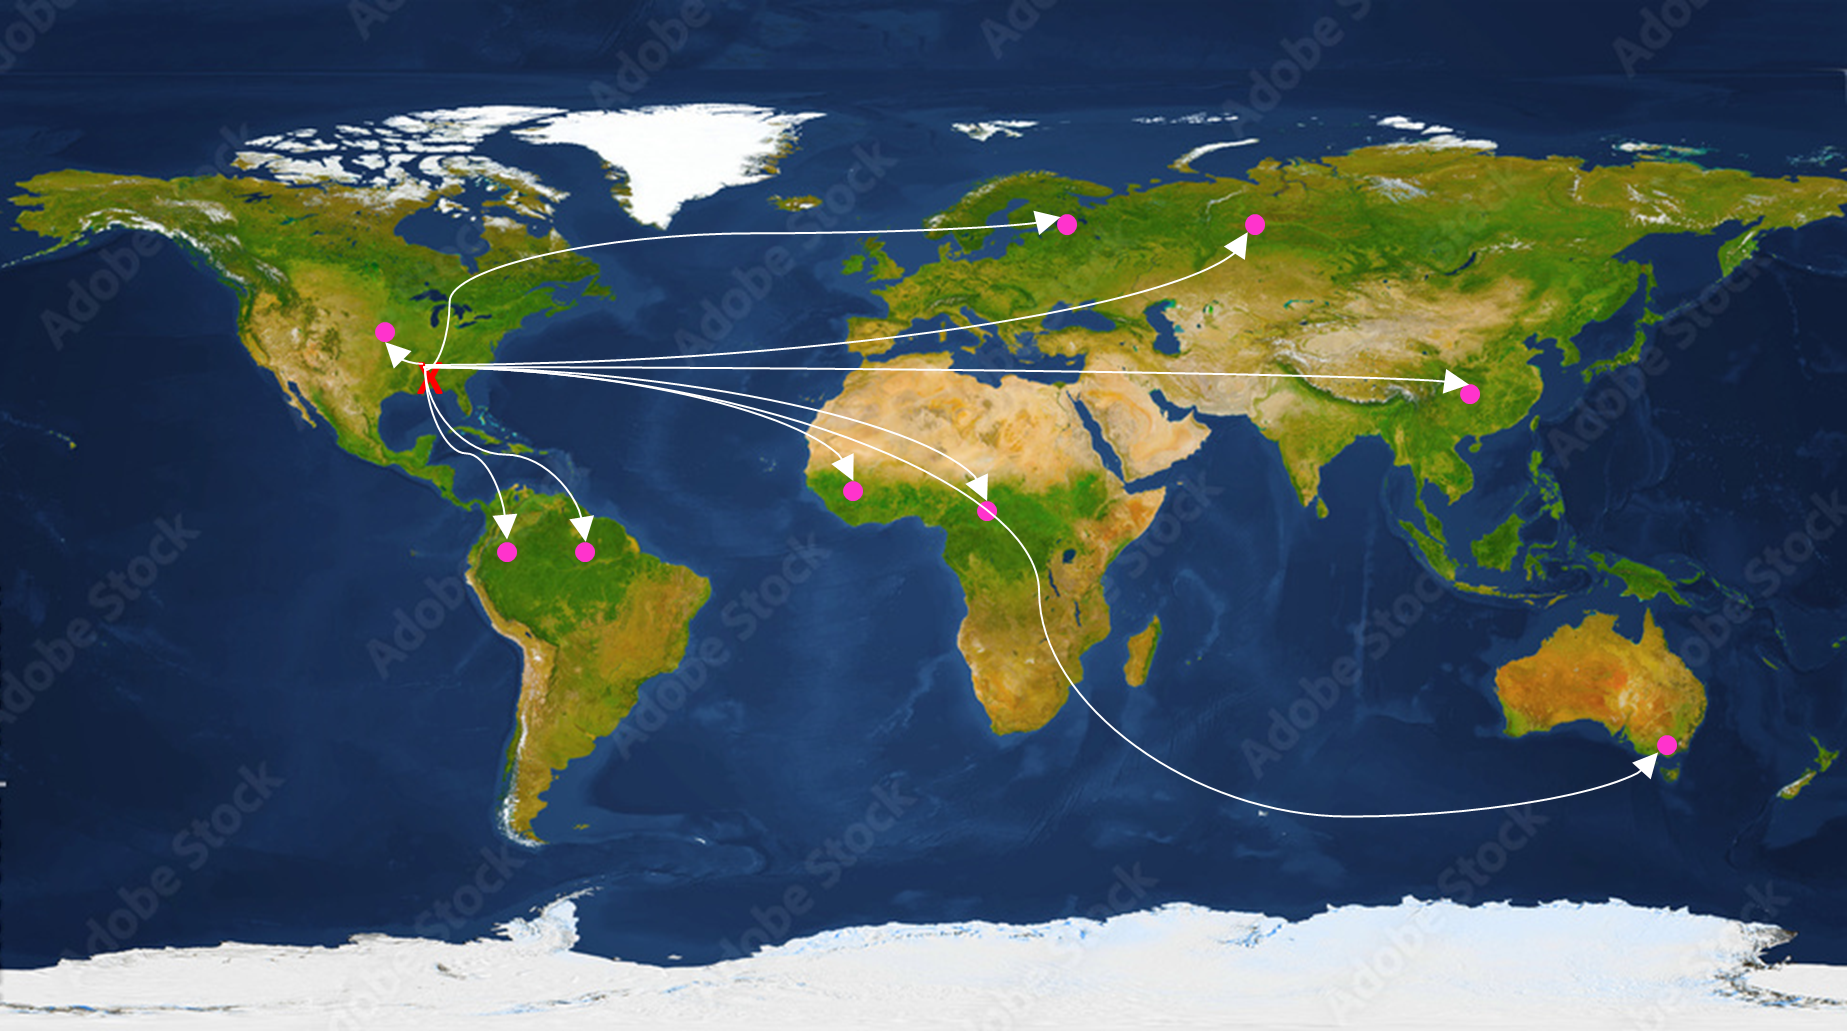
\includegraphics{Figures/Remote_Calibration.png}
\caption{Example of the location of observations (pink circles) that inform the post-processing of rainfall in a specific location (red cross).}
\label{Remote_Calibration}
\end{figure}

%%%%%%%%%%%%%%%%%%%%%%%%%%%%%%%%%%%%%%%%%%%%%%%%%%%%%%%%%%%%%%%%%%%%%%%%%
\subsection{Semi-objective vs automatic calibration approach: on the value of expert elicitation (200 words)}
Lorem ipsum dolor sit amet, consectetur adipiscing elit. Proin vestibulum tincidunt leo. Proin vitae lorem non purus vehicula feugiat. Curabitur quis consectetur nisl. Proin lobortis dictum congue. Nullam sed mattis quam. Nullam sit amet lacus turpis. Ut sed nunc eu nisl varius tristique. Ut fermentum pharetra leo, eget vehicula metus gravida quis. Proin sodales lacus risus, sed iaculis nisi luctus at. Nulla fringilla dapibus tortor, in blandit justo blandit at. Quisque sit amet leo nisl. Donec tempus orci enim, eu porttitor lacus porta nec. Orci varius natoque penatibus et magnis dis parturient montes, nascetur ridiculus mus. Nam a purus sagittis, sollicitudin libero sit amet, commodo arcu. Aliquam erat volutpat. Aenean ut est porttitor, lobortis dui at, facilisis sapien. Proin dapibus leo in blandit posuere. Fusce fringilla sem mattis sapien euismod, eget imperdiet enim vehicula. Suspendisse sem sapien, congue at sapien at, pretium vehicula purus. Vestibulum sed suscipit mauris. Ut id elit ligula. Maecenas a fermentum dolor, quis gravida lorem. Nam convallis pharetra purus. Mauris sapien eros, ultricies quis felis at, interdum mattis augue. Nullam iaculis suscipit condimentum. Curabitur libero sapien, porttitor eu sapien a, elementum hendrerit tellus. Duis arcu nibh, feugiat ut mi in, finibus sodales dui. Curabitur vehicula lorem.. Vestibulum molestie pretium ultrices. Nunc finibus condimentum lectus sit amet tincidunt. Vivamus dignissim ex eget pretium egestas.

%%%%%%%%%%%%%%%%%%%%%%%%%%%%%%%%%%%%%%%%%%%%%%%%%%%%%%%%%%%%%%%%%%%%%%%%%
\subsection{Reproducible calibration results (200 words)}
Lorem ipsum dolor sit amet, consectetur adipiscing elit. Proin vestibulum tincidunt leo. Proin vitae lorem non purus vehicula feugiat. Curabitur quis consectetur nisl. Proin lobortis dictum congue. Nullam sed mattis quam. Nullam sit amet lacus turpis. Ut sed nunc eu nisl varius tristique. Ut fermentum pharetra leo, eget vehicula metus gravida quis. Proin sodales lacus risus, sed iaculis nisi luctus at. Nulla fringilla dapibus tortor, in blandit justo blandit at. Quisque sit amet leo nisl. Donec tempus orci enim, eu porttitor lacus porta nec. Orci varius natoque penatibus et magnis dis parturient montes, nascetur ridiculus mus. Nam a purus sagittis, sollicitudin libero sit amet, commodo arcu. Aliquam erat volutpat. Aenean ut est porttitor, lobortis dui at, facilisis sapien. Proin dapibus leo in blandit posuere. Fusce fringilla sem mattis sapien euismod, eget imperdiet enim vehicula. Suspendisse sem sapien, congue at sapien at, pretium vehicula purus. Vestibulum sed suscipit mauris. Ut id elit ligula. Maecenas a fermentum dolor, quis gravida lorem. Nam convallis pharetra purus. Mauris sapien eros, ultricies quis felis at, interdum mattis augue. Nullam iaculis suscipit condimentum. Curabitur libero sapien, porttitor eu sapien a, elementum hendrerit tellus. Duis arcu nibh, feugiat ut mi in, finibus sodales dui. Curabitur vehicula lorem.. Vestibulum molestie pretium ultrices. Nunc finibus condimentum lectus sit amet tincidunt. Vivamus dignissim ex eget pretium egestas.

\begin{figure}
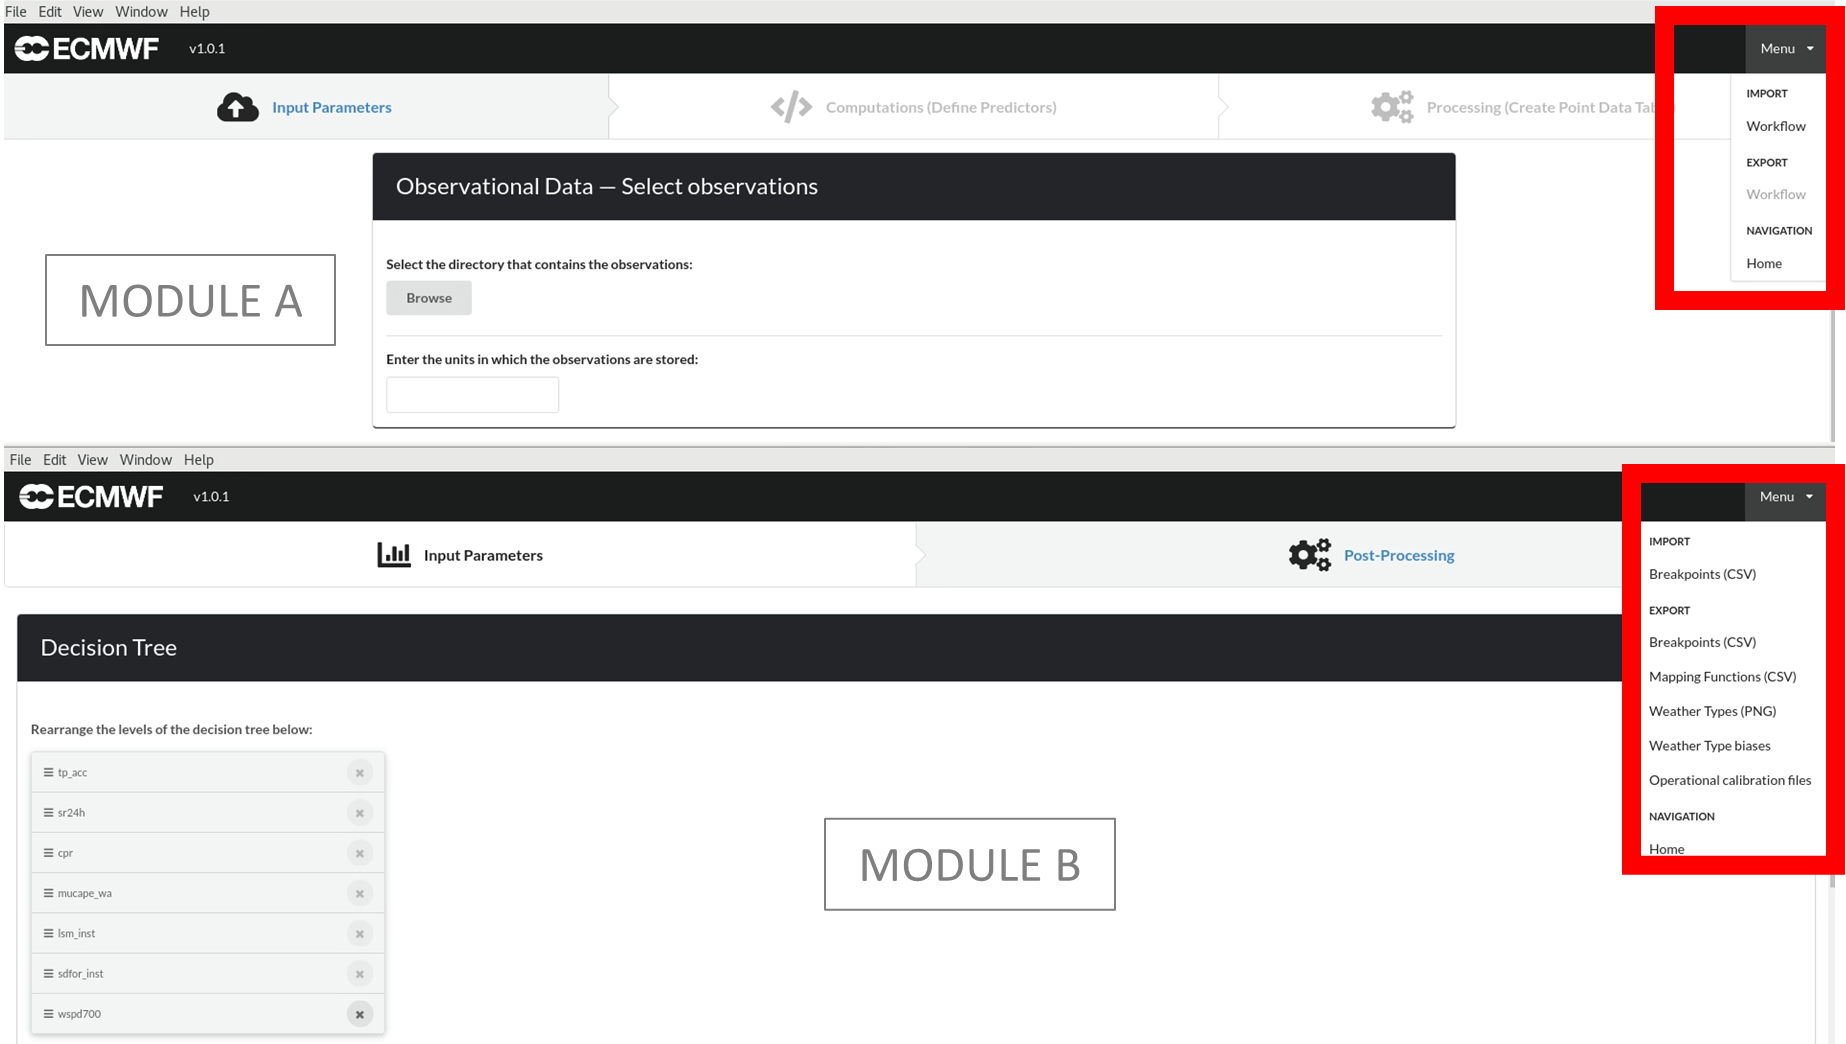
\includegraphics{Figures/Reproducible_Results.png}
\caption{Screenshots of the menu options availbale to users in the different modules of the software to import/export previous results and create reproducible workflows).}
\label{Reproducible_Results}
\end{figure}

%%%%%%%%%%%%%%%%%%%%%%%%%%%%%%%%%%%%%%%%%%%%%%%%%%%%%%%%%%%%%%%%%%%%%%%%%
\subsection{Capability to handle large volumes of data (200 words)}
Lorem ipsum dolor sit amet, consectetur adipiscing elit. Proin vestibulum tincidunt leo. Proin vitae lorem non purus vehicula feugiat. Curabitur quis consectetur nisl. Proin lobortis dictum congue. Nullam sed mattis quam. Nullam sit amet lacus turpis. Ut sed nunc eu nisl varius tristique. Ut fermentum pharetra leo, eget vehicula metus gravida quis. Proin sodales lacus risus, sed iaculis nisi luctus at. Nulla fringilla dapibus tortor, in blandit justo blandit at. Quisque sit amet leo nisl. Donec tempus orci enim, eu porttitor lacus porta nec. Orci varius natoque penatibus et magnis dis parturient montes, nascetur ridiculus mus. Nam a purus sagittis, sollicitudin libero sit amet, commodo arcu. Aliquam erat volutpat. Aenean ut est porttitor, lobortis dui at, facilisis sapien. Proin dapibus leo in blandit posuere. Fusce fringilla sem mattis sapien euismod, eget imperdiet enim vehicula. Suspendisse sem sapien, congue at sapien at, pretium vehicula purus. Vestibulum sed suscipit mauris. Ut id elit ligula. Maecenas a fermentum dolor, quis gravida lorem. Nam convallis pharetra purus. Mauris sapien eros, ultricies quis felis at, interdum mattis augue. Nullam iaculis suscipit condimentum. Curabitur libero sapien, porttitor eu sapien a, elementum hendrerit tellus. Duis arcu nibh, feugiat ut mi in, finibus sodales dui. Curabitur vehicula lorem.. Vestibulum molestie pretium ultrices. Nunc finibus condimentum lectus sit amet tincidunt. Vivamus dignissim ex eget pretium egestas.

%%%%%%%%%%%%%%%%%%%%%%%%%%%%%%%%%%%%%%%%%%%%%%%%%%%%%%%%%%%%%%%%%%%%%%%%%
\subsection{User-friendly GUI (200 words)}
Lorem ipsum dolor sit amet, consectetur adipiscing elit. Proin vestibulum tincidunt leo. Proin vitae lorem non purus vehicula feugiat. Curabitur quis consectetur nisl. Proin lobortis dictum congue. Nullam sed mattis quam. Nullam sit amet lacus turpis. Ut sed nunc eu nisl varius tristique. Ut fermentum pharetra leo, eget vehicula metus gravida quis. Proin sodales lacus risus, sed iaculis nisi luctus at. Nulla fringilla dapibus tortor, in blandit justo blandit at. Quisque sit amet leo nisl. Donec tempus orci enim, eu porttitor lacus porta nec. Orci varius natoque penatibus et magnis dis parturient montes, nascetur ridiculus mus. Nam a purus sagittis, sollicitudin libero sit amet, commodo arcu. Aliquam erat volutpat. Aenean ut est porttitor, lobortis dui at, facilisis sapien. Proin dapibus leo in blandit posuere. Fusce fringilla sem mattis sapien euismod, eget imperdiet enim vehicula. Suspendisse sem sapien, congue at sapien at, pretium vehicula purus. Vestibulum sed suscipit mauris. Ut id elit ligula. Maecenas a fermentum dolor, quis gravida lorem. Nam convallis pharetra purus. Mauris sapien eros, ultricies quis felis at, interdum mattis augue. Nullam iaculis suscipit condimentum. Curabitur libero sapien, porttitor eu sapien a, elementum hendrerit tellus. Duis arcu nibh, feugiat ut mi in, finibus sodales dui. Curabitur vehicula lorem.. Vestibulum molestie pretium ultrices. Nunc finibus condimentum lectus sit amet tincidunt. Vivamus dignissim ex eget pretium egestas.

%%%%%%%%%%%%%%%%%%%%%%%%%%%%%%%%%%%%%%%%%%%%%%%%%%%%%%%%%%%%%%%%%%%%%%%%%
\section{Post-processing approach}

\subsection{Calibration assumptions, 200 words}
Lorem ipsum dolor sit amet, consectetur adipiscing elit. Morbi elementum orci nec mauris mollis ornare. Pellentesque congue purus sapien, vitae sagittis massa auctor sed. Pellentesque gravida sem eget orci dapibus interdum. Suspendisse vitae libero ut tortor fermentum egestas. Nullam lacinia ultricies dapibus. Nam vitae porttitor turpis, eu hendrerit lectus. Nulla sollicitudin velit et elit porta eleifend. Praesent laoreet eros vitae nibh tempor, bibendum lacinia ante rhoncus. Pellentesque consequat in diam non porta. Nunc sollicitudin purus et molestie suscipit. Curabitur aliquam ipsum vel ligula facilisis ullamcorper. Donec sollicitudin sapien in dui lobortis, et efficitur tortor dictum. Nullam eu semper elit, a lacinia nulla. Cras nec interdum arcu. Sed non scelerisque urna, non viverra ante. Cras elementum justo ut mi porttitor fringilla sit amet sed mauris. Vestibulum ac ex venenatis, malesuada quam venenatis, semper ipsum. Cras ac lorem quis nisi porta pharetra ut venenatis erat. Curabitur a aliquet metus. Phasellus vitae lectus.

%%%%%%%%%%%%%%%%%%%%%%%%%%%%%%%%%%%%%%%%%%%%%%%%%%%%%%%%%%%%%%%%%%%%%%%%%
\subsection{Mapping functions, 200 words}
Lorem ipsum dolor sit amet, consectetur adipiscing elit. Morbi elementum orci nec mauris mollis ornare. Pellentesque congue purus sapien, vitae sagittis massa auctor sed. Pellentesque gravida sem eget orci dapibus interdum. Suspendisse vitae libero ut tortor fermentum egestas. Nullam lacinia ultricies dapibus. Nam vitae porttitor turpis, eu hendrerit lectus. Nulla sollicitudin velit et elit porta eleifend. Praesent laoreet eros vitae nibh tempor, bibendum lacinia ante rhoncus. Pellentesque consequat in diam non porta. Nunc sollicitudin purus et molestie suscipit. Curabitur aliquam ipsum vel ligula facilisis ullamcorper. Donec sollicitudin sapien in dui lobortis, et efficitur tortor dictum. Nullam eu semper elit, a lacinia nulla. Cras nec interdum arcu. Sed non scelerisque urna, non viverra ante. Cras elementum justo ut mi porttitor fringilla sit amet sed mauris. Vestibulum ac ex venenatis, malesuada quam venenatis, semper ipsum. Cras ac lorem quis nisi porta pharetra ut venenatis erat. Curabitur a aliquet metus. Phasellus vitae lectus.

\begin{figure}
\centering
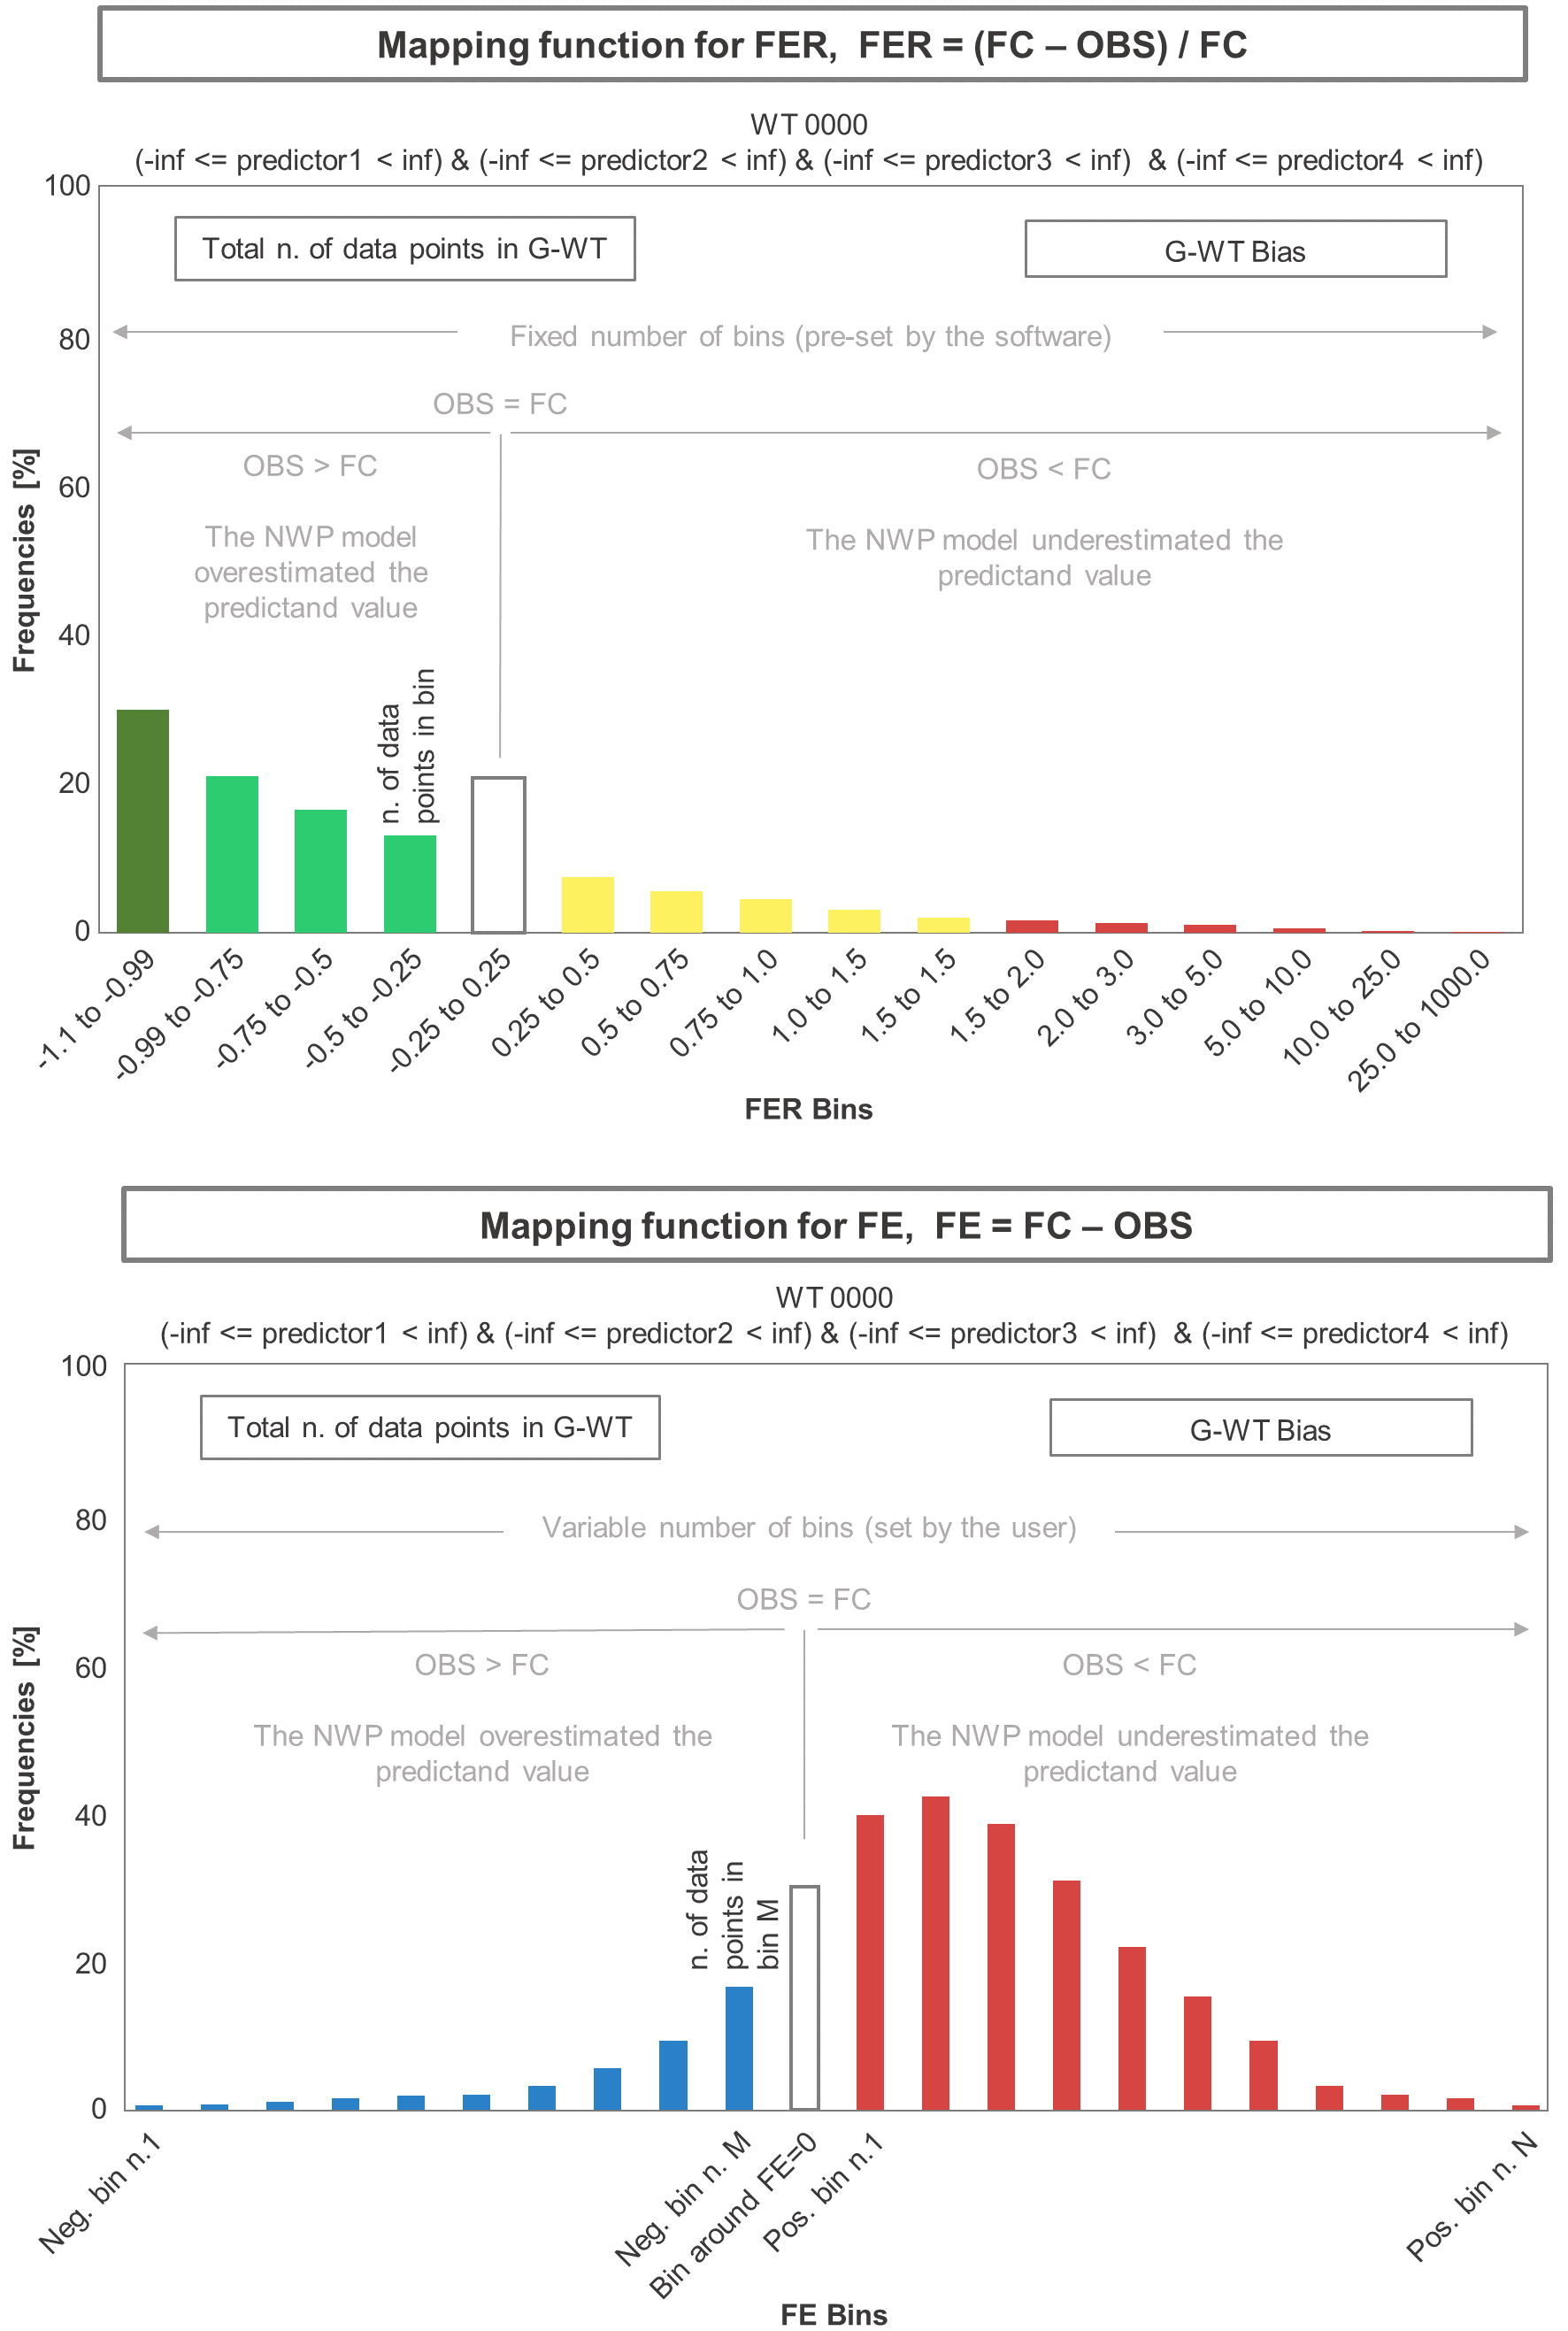
\includegraphics{Figures/Examples_MF.png}
\caption{Example of mapping function (MF) for Forecast Error Ratio (FER, top panel) and Forecast Error (FE, bottom panel).}
\label{Examples_MF}
\end{figure}

%%%%%%%%%%%%%%%%%%%%%%%%%%%%%%%%%%%%%%%%%%%%%%%%%%%%%%%%%%%%%%%%%%%%%%%%%
\section{ecPoint-Calibrate workflow, 100 words}

Lorem ipsum dolor sit amet, consectetur adipiscing elit. Nulla finibus dignissim nibh eget sodales. Pellentesque nunc ex, euismod nec velit non, interdum bibendum mi. Sed quis nisl et tortor congue vulputate. Quisque feugiat interdum finibus. Etiam pellentesque nunc nec neque vestibulum condimentum. Pellentesque quis sapien at purus fringilla gravida. Sed accumsan risus nec libero pretium cursus. Sed eu viverra tortor. Nam lacinia arcu quis lobortis viverra. Sed mollis et ex vitae convallis. Sed metus enim, dictum eget condimentum sed, tincidunt quis erat. Phasellus at turpis vitae quam malesuada eleifend. In in sagittis turpis. Aenean ullamcorper dolor et erat facilisis, id.

\begin{figure}
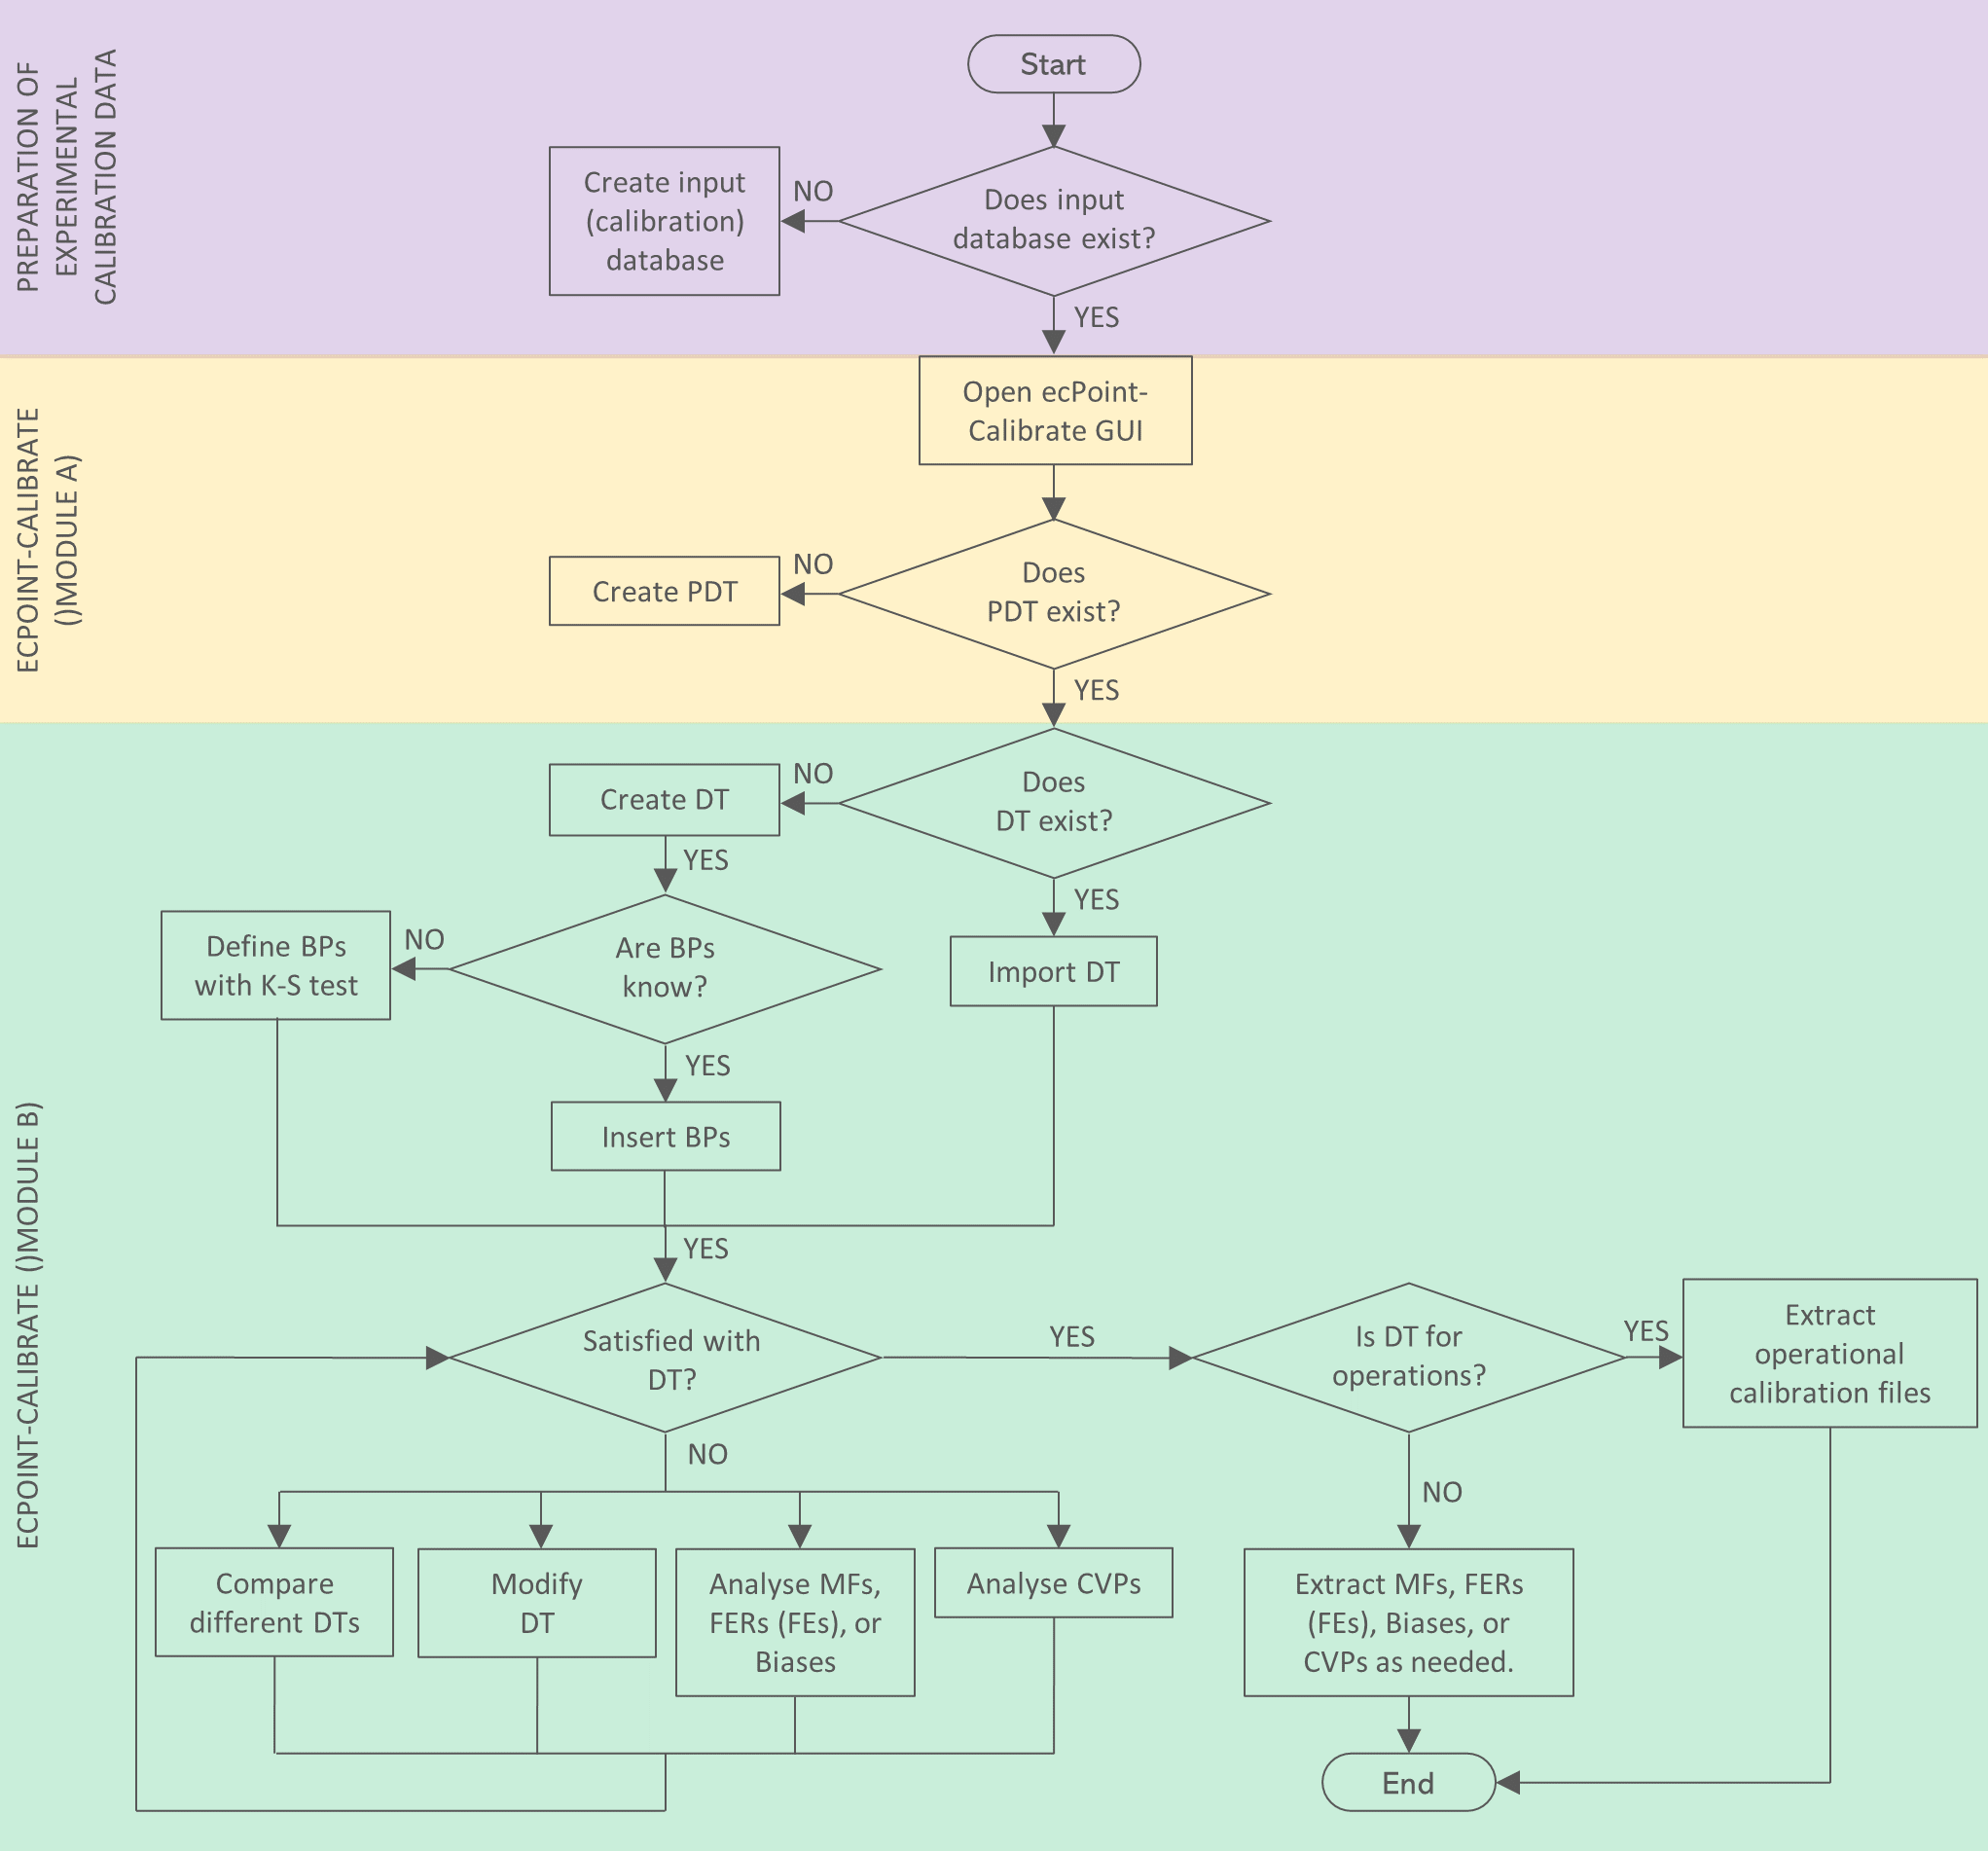
\includegraphics{Figures/Flowchart_ecPointCalibrate_Workflow.png}
\caption{ecPoint-Calibrate workflow}
\label{Flowchart_ecPointCalibrate_Workflow}
\end{figure}

%%%%%%%%%%%%%%%%%%%%%%%%%%%%%%%%%%%%%%%%%%%%%%%%%%%%%%%%%%%%%%%%%%%%%%%%%
\subsection{Creating the input database, 200 words}

Lorem ipsum dolor sit amet, consectetur adipiscing elit. Proin vestibulum tincidunt leo. Proin vitae lorem non purus vehicula feugiat. Curabitur quis consectetur nisl. Proin lobortis dictum congue. Nullam sed mattis quam. Nullam sit amet lacus turpis. Ut sed nunc eu nisl varius tristique. Ut fermentum pharetra leo, eget vehicula metus gravida quis. Proin sodales lacus risus, sed iaculis nisi luctus at. Nulla fringilla dapibus tortor, in blandit justo blandit at. Quisque sit amet leo nisl. Donec tempus orci enim, eu porttitor lacus porta nec. Orci varius natoque penatibus et magnis dis parturient montes, nascetur ridiculus mus. Nam a purus sagittis, sollicitudin libero sit amet, commodo arcu. Aliquam erat volutpat. Aenean ut est porttitor, lobortis dui at, facilisis sapien. Proin dapibus leo in blandit posuere. Fusce fringilla sem mattis sapien euismod, eget imperdiet enim vehicula. Suspendisse sem sapien, congue at sapien at, pretium vehicula purus. Vestibulum sed suscipit mauris. Ut id elit ligula. Maecenas a fermentum dolor, quis gravida lorem. Nam convallis pharetra purus. Mauris sapien eros, ultricies quis felis at, interdum mattis augue. Nullam iaculis suscipit condimentum. Curabitur libero sapien, porttitor eu sapien a, elementum hendrerit tellus. Duis arcu nibh, feugiat ut mi in, finibus sodales dui. Curabitur 

\begin{figure}
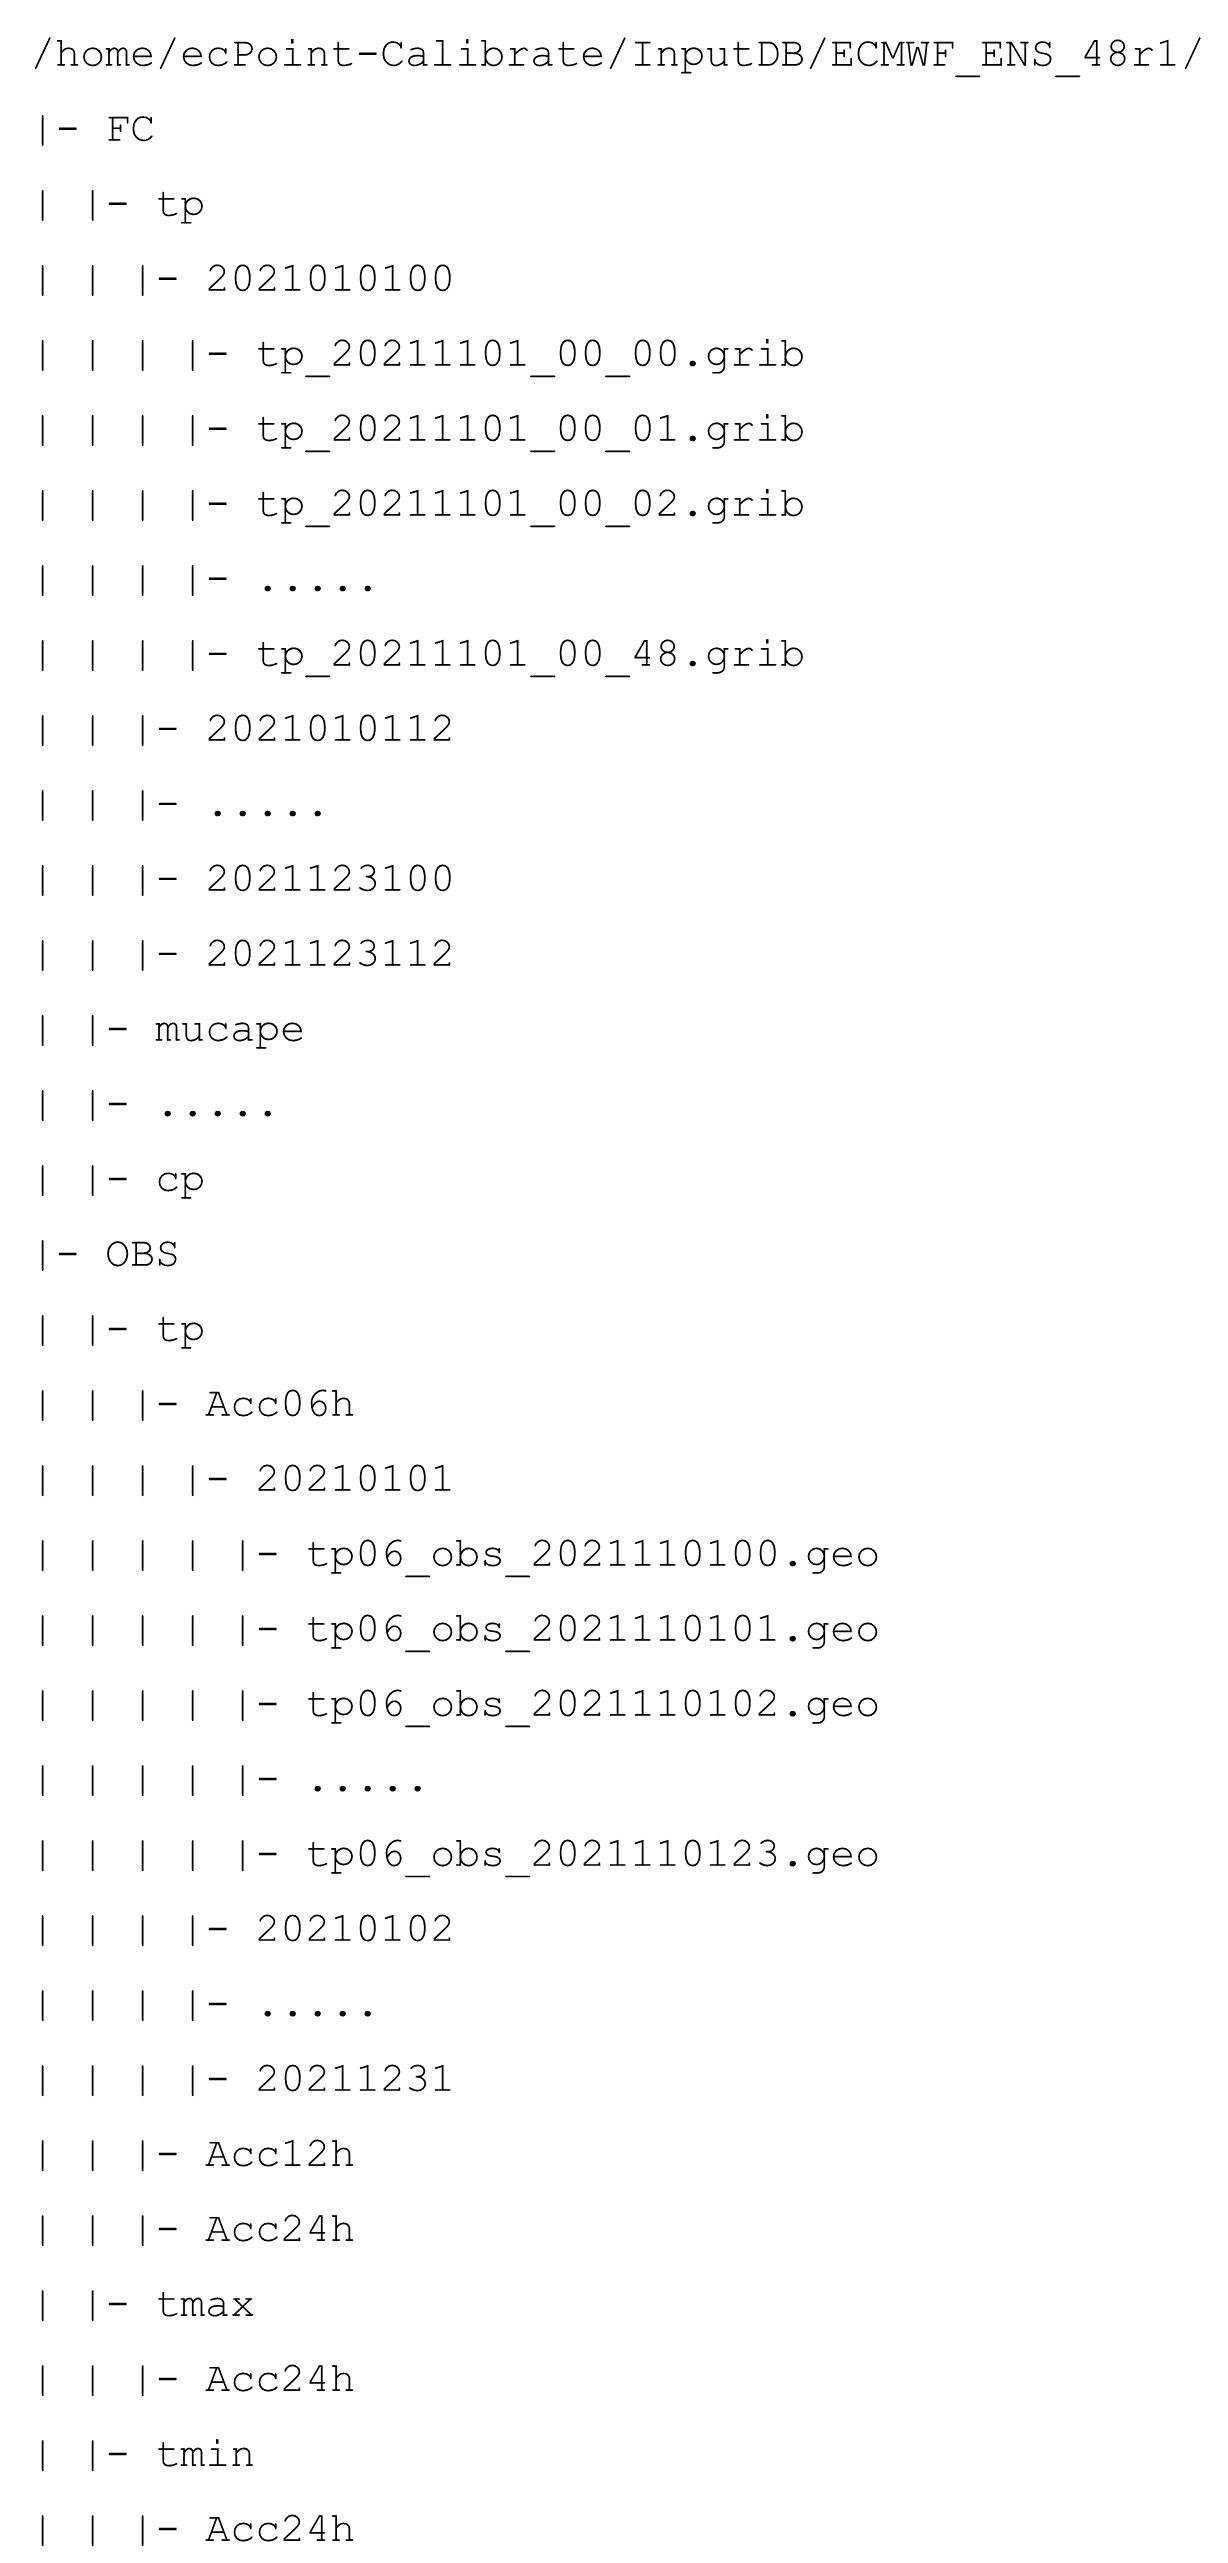
\includegraphics{Figures/Input_Database.png}
\caption{Organization of the input database}
\label{Input_Database}
\end{figure}

%%%%%%%%%%%%%%%%%%%%%%%%%%%%%%%%%%%%%%%%%%%%%%%%%%%%%%%%%%%%%%%%%%%%%%%%%
\subsection{Generation of the point data table: Module A}

\subsubsection{Part 1: Input Parameters, 100 words}
Lorem ipsum dolor sit amet, consectetur adipiscing elit. Maecenas sed ligula volutpat, iaculis massa nec, facilisis sem. Nulla accumsan convallis lectus, at porttitor sem. Vestibulum tincidunt nunc a risus vestibulum aliquam vitae in nibh. Nam vitae fringilla felis. Cras hendrerit mauris id arcu volutpat, vitae porta nunc elementum. Sed mauris magna, sodales et massa in, rhoncus pharetra leo. In et velit a nibh aliquam fermentum. Proin eu lorem in mauris scelerisque ultricies et vitae lectus. Lorem ipsum dolor sit amet, consectetur adipiscing elit. Aliquam maximus hendrerit tempus. Pellentesque nec tristique tellus, nec molestie nunc. In iaculis nisi eu lorem venenatis lobortis. Nunc euismod lorem quis blandit suscipit. Sed non tempor arcu. Aenean pharetra ut turpis sed fermentum. Duis egestas nisi sit amet metus ornare facilisis. Quisque enim nisi, eleifend at cursus sit amet, suscipit id ex. Nam condimentum, arcu et ultricies egestas, mi urna commodo massa, eget venenatis nulla purus.




%%%%%%%%%%%%%%%%%%%%%%%%%%%%%%%%%%%%%%%%%%%%%%%%%%%%%%%%%%%%%%%%%%%%%%%%%
\subsubsection{Part 2: Computations (Define Predictors), 100 words}
Lorem ipsum dolor sit amet, consectetur adipiscing elit. Maecenas sed ligula volutpat, iaculis massa nec, facilisis sem. Nulla accumsan convallis lectus, at porttitor sem. Vestibulum tincidunt nunc a risus vestibulum aliquam vitae in nibh. Nam vitae fringilla felis. Cras hendrerit mauris id arcu volutpat, vitae porta nunc elementum. Sed mauris magna, sodales et massa in, rhoncus pharetra leo. In et velit a nibh aliquam fermentum. Proin eu lorem in mauris scelerisque ultricies et vitae lectus. Lorem ipsum dolor sit amet, consectetur adipiscing elit. Aliquam maximus hendrerit tempus. Pellentesque nec tristique tellus, nec molestie nunc. In iaculis nisi eu lorem venenatis lobortis. Nunc euismod lorem quis blandit suscipit. Sed non tempor arcu. Aenean pharetra ut turpis sed fermentum. Duis egestas nisi sit amet metus ornare facilisis. Quisque enim nisi, eleifend at cursus sit amet, suscipit id ex. Nam condimentum, arcu et ultricies egestas, mi urna commodo massa, eget venenatis nulla purus.

%%%%%%%%%%%%%%%%%%%%%%%%%%%%%%%%%%%%%%%%%%%%%%%%%%%%%%%%%%%%%%%%%%%%%%%%%
\subsubsection{Part 3: Processing (Creating point data table), 100 words}
Lorem ipsum dolor sit amet, consectetur adipiscing elit. Maecenas sed ligula volutpat, iaculis massa nec, facilisis sem. Nulla accumsan convallis lectus, at porttitor sem. Vestibulum tincidunt nunc a risus vestibulum aliquam vitae in nibh. Nam vitae fringilla felis. Cras hendrerit mauris id arcu volutpat, vitae porta nunc elementum. Sed mauris magna, sodales et massa in, rhoncus pharetra leo. In et velit a nibh aliquam fermentum. Proin eu lorem in mauris scelerisque ultricies et vitae lectus. Lorem ipsum dolor sit amet, consectetur adipiscing elit. Aliquam maximus hendrerit tempus. Pellentesque nec tristique tellus, nec molestie nunc. In iaculis nisi eu lorem venenatis lobortis. Nunc euismod lorem quis blandit suscipit. Sed non tempor arcu. Aenean pharetra ut turpis sed fermentum. Duis egestas nisi sit amet metus ornare facilisis. Quisque enim nisi, eleifend at cursus sit amet, suscipit id ex. Nam condimentum, arcu et ultricies egestas, mi urna commodo massa, eget venenatis nulla purus.

\begin{figure}
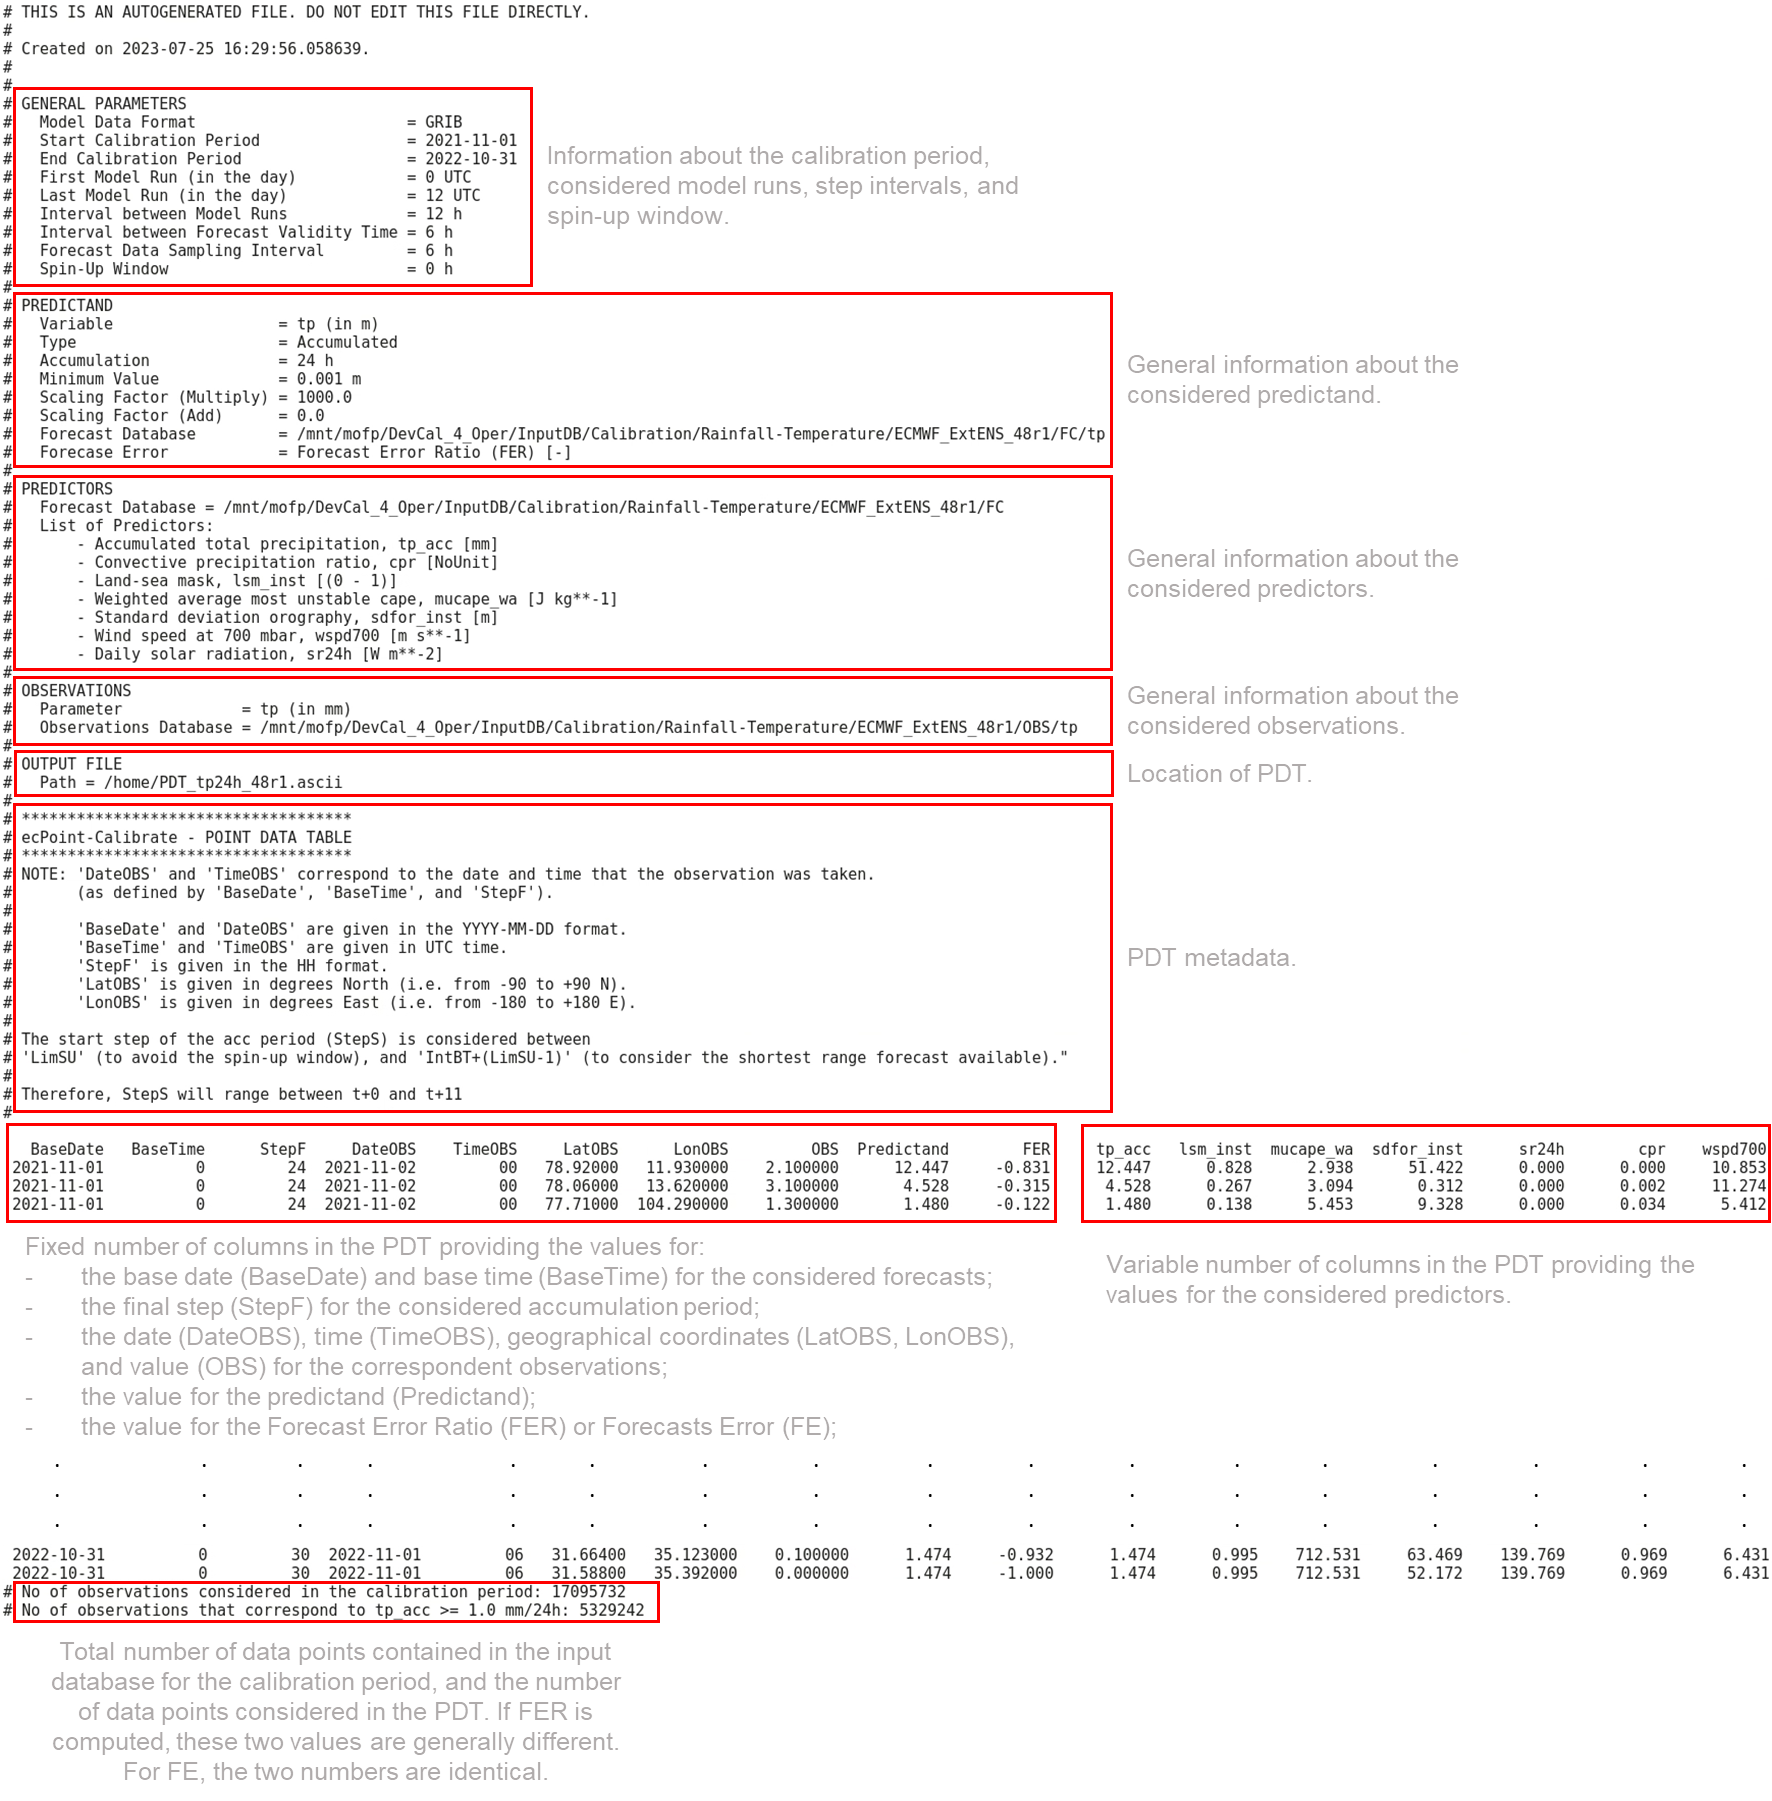
\includegraphics{Figures/Example_PDT.png}
\caption{Example of a point data table (PDT), and description of its internal organization.}
\label{Example_PDT}
\end{figure}

%%%%%%%%%%%%%%%%%%%%%%%%%%%%%%%%%%%%%%%%%%%%%%%%%%%%%%%%%%%%%%%%%%%%%%%%%
\section{Creation of the decision tree and conditional verification plots: Module B}

\subsection{Part 1: Input Parameters, 100 words}
Lorem ipsum dolor sit amet, consectetur adipiscing elit. Nulla finibus dignissim nibh eget sodales. Pellentesque nunc ex, euismod nec velit non, interdum bibendum mi. Sed quis nisl et tortor congue vulputate. Quisque feugiat interdum finibus. Etiam pellentesque nunc nec neque vestibulum condimentum. Pellentesque quis sapien at purus fringilla gravida. Sed accumsan risus nec libero pretium cursus. Sed eu viverra tortor. Nam lacinia arcu quis lobortis viverra. Sed mollis et ex vitae convallis. Sed metus enim, dictum eget condimentum sed, tincidunt quis erat. Phasellus at turpis vitae quam malesuada eleifend. In in sagittis turpis. Aenean ullamcorper dolor et erat facilisis, id.

%%%%%%%%%%%%%%%%%%%%%%%%%%%%%%%%%%%%%%%%%%%%%%%%%%%%%%%%%%%%%%%%%%%%%%%%%
\subsection{Part 2: Post-processing, 100 words}
Lorem ipsum dolor sit amet, consectetur adipiscing elit. Nulla finibus dignissim nibh eget sodales. Pellentesque nunc ex, euismod nec velit non, interdum bibendum mi. Sed quis nisl et tortor congue vulputate. Quisque feugiat interdum finibus. Etiam pellentesque nunc nec neque vestibulum condimentum. Pellentesque quis sapien at purus fringilla gravida. Sed accumsan risus nec libero pretium cursus. Sed eu viverra tortor. Nam lacinia arcu quis lobortis viverra. Sed mollis et ex vitae convallis. Sed metus enim, dictum eget condimentum sed, tincidunt quis erat. Phasellus at turpis vitae quam malesuada eleifend. In in sagittis turpis. Aenean ullamcorper dolor et erat facilisis, id.

%%%%%%%%%%%%%%%%%%%%%%%%%%%%%%%%%%%%%%%%%%%%%%%%%%%%%%%%%%%%%%%%%%%%%%%%%
\subsubsection{Testing the utility of governing variables, 200 words}
Lorem ipsum dolor sit amet, consectetur adipiscing elit. Proin vestibulum tincidunt leo. Proin vitae lorem non purus vehicula feugiat. Curabitur quis consectetur nisl. Proin lobortis dictum congue. Nullam sed mattis quam. Nullam sit amet lacus turpis. Ut sed nunc eu nisl varius tristique. Ut fermentum pharetra leo, eget vehicula metus gravida quis. Proin sodales lacus risus, sed iaculis nisi luctus at. Nulla fringilla dapibus tortor, in blandit justo blandit at. Quisque sit amet leo nisl. Donec tempus orci enim, eu porttitor lacus porta nec. Orci varius natoque penatibus et magnis dis parturient montes, nascetur ridiculus mus. Nam a purus sagittis, sollicitudin libero sit amet, commodo arcu. Aliquam erat volutpat. Aenean ut est porttitor, lobortis dui at, facilisis sapien. Proin dapibus leo in blandit posuere. Fusce fringilla sem mattis sapien euismod, eget imperdiet enim vehicula. Suspendisse sem sapien, congue at sapien at, pretium vehicula purus. Vestibulum sed suscipit mauris. Ut id elit ligula. Maecenas a fermentum dolor, quis gravida lorem. Nam convallis pharetra purus. Mauris sapien eros, ultricies quis felis at, interdum mattis augue. Nullam iaculis suscipit condimentum. Curabitur libero sapien, porttitor eu sapien a, elementum hendrerit tellus. Duis arcu nibh, feugiat ut mi in, finibus sodales dui. Curabitur vehicula lorem.. Vestibulum molestie pretium ultrices. Nunc finibus condimentum lectus sit amet tincidunt. Vivamus dignissim ex eget pretium egestas.

%%%%%%%%%%%%%%%%%%%%%%%%%%%%%%%%%%%%%%%%%%%%%%%%%%%%%%%%%%%%%%%%%%%%%%%%%
\subsection{Building a decision tree, 200 words}
Lorem ipsum dolor sit amet, consectetur adipiscing elit. Proin vestibulum tincidunt leo. Proin vitae lorem non purus vehicula feugiat. Curabitur quis consectetur nisl. Proin lobortis dictum congue. Nullam sed mattis quam. Nullam sit amet lacus turpis. Ut sed nunc eu nisl varius tristique. Ut fermentum pharetra leo, eget vehicula metus gravida quis. Proin sodales lacus risus, sed iaculis nisi luctus at. Nulla fringilla dapibus tortor, in blandit justo blandit at. Quisque sit amet leo nisl. Donec tempus orci enim, eu porttitor lacus porta nec. Orci varius natoque penatibus et magnis dis parturient montes, nascetur ridiculus mus. Nam a purus sagittis, sollicitudin libero sit amet, commodo arcu. Aliquam erat volutpat. Aenean ut est porttitor, lobortis dui at, facilisis sapien. Proin dapibus leo in blandit posuere. Fusce fringilla sem mattis sapien euismod, eget imperdiet enim vehicula. Suspendisse sem sapien, congue at sapien at, pretium vehicula purus. Vestibulum sed suscipit mauris. Ut id elit ligula. Maecenas a fermentum dolor, quis gravida lorem. Nam convallis pharetra purus. Mauris sapien eros, ultricies quis felis at, interdum mattis augue. Nullam iaculis suscipit condimentum. Curabitur libero sapien, porttitor eu sapien a, elementum hendrerit tellus. Duis arcu nibh, feugiat ut mi in, finibus sodales dui. Curabitur vehicula lorem.. Vestibulum molestie pretium ultrices. Nunc finibus condimentum lectus sit amet tincidunt. Vivamus dignissim ex eget pretium egestas.

%%%%%%%%%%%%%%%%%%%%%%%%%%%%%%%%%%%%%%%%%%%%%%%%%%%%%%%%%%%%%%%%%%%%%%%%%
\subsection{Creating conditional verification plots, 150 words}
Lorem ipsum dolor sit amet, consectetur adipiscing elit. Proin vestibulum tincidunt leo. Proin vitae lorem non purus vehicula feugiat. Curabitur quis consectetur nisl. Proin lobortis dictum congue. Nullam sed mattis quam. Nullam sit amet lacus turpis. Ut sed nunc eu nisl varius tristique. Ut fermentum pharetra leo, eget vehicula metus gravida quis. Proin sodales lacus risus, sed iaculis nisi luctus at. Nulla fringilla dapibus tortor, in blandit justo blandit at. Quisque sit amet leo nisl. Donec tempus orci enim, eu porttitor lacus porta nec. Orci varius natoque penatibus et magnis dis parturient montes, nascetur ridiculus mus. Nam a purus sagittis, sollicitudin libero sit amet, commodo arcu. Aliquam erat volutpat. Aenean ut est porttitor, lobortis dui at, facilisis sapien. Proin dapibus leo in blandit posuere. Fusce fringilla sem mattis sapien euismod, eget imperdiet enim vehicula. Suspendisse sem sapien, congue at sapien at, pretium vehicula purus. Vestibulum sed suscipit mauris. Ut id elit ligula. Maecenas a fermentum dolor, quis gravida lorem. Nam convallis pharetra purus. Mauris sapien eros, ultricies quis felis at, interdum mattis augue. Nullam iaculis suscipit condimentum. Curabitur libero sapien, porttitor eu sapien a, elementum hendrerit tellus. Duis arcu nibh, feugiat ut mi in, finibus sodales dui. Curabitur vehicula lorem.. Vestibulum molestie pretium ultrices. Nunc finibus condimentum lectus sit amet tincidunt. Vivamus dignissim ex eget pretium egestas.

%%%%%%%%%%%%%%%%%%%%%%%%%%%%%%%%%%%%%%%%%%%%%%%%%%%%%%%%%%%%%%%%%%%%%%%%%
\section{Software outputs (200 words)}
Lorem ipsum dolor sit amet, consectetur adipiscing elit. Proin vestibulum tincidunt leo. Proin vitae lorem non purus vehicula feugiat. Curabitur quis consectetur nisl. Proin lobortis dictum congue. Nullam sed mattis quam. Nullam sit amet lacus turpis. Ut sed nunc eu nisl varius tristique. Ut fermentum pharetra leo, eget vehicula metus gravida quis. Proin sodales lacus risus, sed iaculis nisi luctus at. Nulla fringilla dapibus tortor, in blandit justo blandit at. Quisque sit amet leo nisl. Donec tempus orci enim, eu porttitor lacus porta nec. Orci varius natoque penatibus et magnis dis parturient montes, nascetur ridiculus mus. Nam a purus sagittis, sollicitudin libero sit amet, commodo arcu. Aliquam erat volutpat. Aenean ut est porttitor, lobortis dui at, facilisis sapien. Proin dapibus leo in blandit posuere. Fusce fringilla sem mattis sapien euismod, eget imperdiet enim vehicula. Suspendisse sem sapien, congue at sapien at, pretium vehicula purus. Vestibulum sed suscipit mauris. Ut id elit ligula. Maecenas a fermentum dolor, quis gravida lorem. Nam convallis pharetra purus. Mauris sapien eros, ultricies quis felis at, interdum mattis augue. Nullam iaculis suscipit condimentum. Curabitur libero sapien, porttitor eu sapien a, elementum hendrerit tellus. Duis arcu nibh, feugiat ut mi in, finibus sodales dui. Curabitur vehicula lorem.. Vestibulum molestie pretium ultrices. Nunc finibus condimentum lectus sit amet tincidunt. Vivamus dignissim ex eget pretium egestas.

%%%%%%%%%%%%%%%%%%%%%%%%%%%%%%%%%%%%%%%%%%%%%%%%%%%%%%%%%%%%%%%%%%%%%%%%%
\section{Downstream use-cases of ecPoint-Calibrate}
\subsection{Analyzes of model characteristics: biases and sub-grid variability, 100 words}
Lorem ipsum dolor sit amet, consectetur adipiscing elit. Nulla finibus dignissim nibh eget sodales. Pellentesque nunc ex, euismod nec velit non, interdum bibendum mi. Sed quis nisl et tortor congue vulputate. Quisque feugiat interdum finibus. Etiam pellentesque nunc nec neque vestibulum condimentum. Pellentesque quis sapien at purus fringilla gravida. Sed accumsan risus nec libero pretium cursus. Sed eu viverra tortor. Nam lacinia arcu quis lobortis viverra. Sed mollis et ex vitae convallis. Sed metus enim, dictum eget condimentum sed, tincidunt quis erat. Phasellus at turpis vitae quam malesuada eleifend. In in sagittis turpis. Aenean ullamcorper dolor et erat facilisis, id.

%%%%%%%%%%%%%%%%%%%%%%%%%%%%%%%%%%%%%%%%%%%%%%%%%%%%%%%%%%%%%%%%%%%%%%%%%
\subsection{Comparison of the characteristics of two model versions, 100 words}
Lorem ipsum dolor sit amet, consectetur adipiscing elit. Nulla finibus dignissim nibh eget sodales. Pellentesque nunc ex, euismod nec velit non, interdum bibendum mi. Sed quis nisl et tortor congue vulputate. Quisque feugiat interdum finibus. Etiam pellentesque nunc nec neque vestibulum condimentum. Pellentesque quis sapien at purus fringilla gravida. Sed accumsan risus nec libero pretium cursus. Sed eu viverra tortor. Nam lacinia arcu quis lobortis viverra. Sed mollis et ex vitae convallis. Sed metus enim, dictum eget condimentum sed, tincidunt quis erat. Phasellus at turpis vitae quam malesuada eleifend. In in sagittis turpis. Aenean ullamcorper dolor et erat facilisis, id.

%%%%%%%%%%%%%%%%%%%%%%%%%%%%%%%%%%%%%%%%%%%%%%%%%%%%%%%%%%%%%%%%%%%%%%%%%
\subsection{Post-processing rainfall and temperature forecasts, 100 words}
Lorem ipsum dolor sit amet, consectetur adipiscing elit. Nulla finibus dignissim nibh eget sodales. Pellentesque nunc ex, euismod nec velit non, interdum bibendum mi. Sed quis nisl et tortor congue vulputate. Quisque feugiat interdum finibus. Etiam pellentesque nunc nec neque vestibulum condimentum. Pellentesque quis sapien at purus fringilla gravida. Sed accumsan risus nec libero pretium cursus. Sed eu viverra tortor. Nam lacinia arcu quis lobortis viverra. Sed mollis et ex vitae convallis. Sed metus enim, dictum eget condimentum sed, tincidunt quis erat. Phasellus at turpis vitae quam malesuada eleifend. In in sagittis turpis. Aenean ullamcorper dolor et erat facilisis, id.

%%%%%%%%%%%%%%%%%%%%%%%%%%%%%%%%%%%%%%%%%%%%%%%%%%%%%%%%%%%%%%%%%%%%%%%%%
\section{Summary, 200 words}
Lorem ipsum dolor sit amet, consectetur adipiscing elit. Proin vestibulum tincidunt leo. Proin vitae lorem non purus vehicula feugiat. Curabitur quis consectetur nisl. Proin lobortis dictum congue. Nullam sed mattis quam. Nullam sit amet lacus turpis. Ut sed nunc eu nisl varius tristique. Ut fermentum pharetra leo, eget vehicula metus gravida quis. Proin sodales lacus risus, sed iaculis nisi luctus at. Nulla fringilla dapibus tortor, in blandit justo blandit at. Quisque sit amet leo nisl. Donec tempus orci enim, eu porttitor lacus porta nec. Orci varius natoque penatibus et magnis dis parturient montes, nascetur ridiculus mus. Nam a purus sagittis, sollicitudin libero sit amet, commodo arcu. Aliquam erat volutpat. Aenean ut est porttitor, lobortis dui at, facilisis sapien. Proin dapibus leo in blandit posuere. Fusce fringilla sem mattis sapien euismod, eget imperdiet enim vehicula. Suspendisse sem sapien, congue at sapien at, pretium vehicula purus. Vestibulum sed suscipit mauris. Ut id elit ligula. Maecenas a fermentum dolor, quis gravida lorem. Nam convallis pharetra purus. Mauris sapien eros, ultricies quis felis at, interdum mattis augue. Nullam iaculis suscipit condimentum. Curabitur libero sapien, porttitor eu sapien a, elementum hendrerit tellus. Duis arcu nibh, feugiat ut mi in, finibus sodales dui. Curabitur vehicula lorem.. Vestibulum molestie pretium ultrices. Nunc finibus condimentum lectus sit amet tincidunt. Vivamus dignissim ex eget pretium egestas.

%%%%%%%%%%%%%%%%%%%%%%%%%%%%%%%%%%%%%%%%%%%%%%%%%%%%%%%%%%%%%%%%%%%%%%%%%
\section{Software availability, 100 words}
Lorem ipsum dolor sit amet, consectetur adipiscing elit. Nulla finibus dignissim nibh eget sodales. Pellentesque nunc ex, euismod nec velit non, interdum bibendum mi. Sed quis nisl et tortor congue vulputate. Quisque feugiat interdum finibus. Etiam pellentesque nunc nec neque vestibulum condimentum. Pellentesque quis sapien at purus fringilla gravida. Sed accumsan risus nec libero pretium cursus. Sed eu viverra tortor. Nam lacinia arcu quis lobortis viverra. Sed mollis et ex vitae convallis. Sed metus enim, dictum eget condimentum sed, tincidunt quis erat. Phasellus at turpis vitae quam malesuada eleifend. In in sagittis turpis. Aenean ullamcorper dolor et erat facilisis, id.

%%%%%%%%%%%%%%%%%%%%%%%%%%%%%%%%%%%%%%%%%%%%%%%%%%%%%%%%%%%%%%%%%%%%%%%%%
\section*{Acknowledgements}
Lorem ipsum dolor sit amet, consectetur adipiscing elit. Morbi elementum orci nec mauris mollis ornare. Pellentesque congue purus sapien, vitae sagittis massa auctor sed. Pellentesque gravida sem eget orci dapibus interdum. Suspendisse vitae libero ut tortor fermentum egestas. Nullam lacinia ultricies dapibus. Nam vitae porttitor turpis, eu hendrerit lectus. Nulla sollicitudin velit et elit porta eleifend. Praesent laoreet eros vitae nibh tempor, bibendum lacinia ante rhoncus. Pellentesque consequat in diam non porta. Nunc sollicitudin purus et molestie suscipit. Curabitur aliquam ipsum vel ligula facilisis ullamcorper. Donec sollicitudin sapien in dui lobortis, et efficitur tortor dictum. Nullam eu semper elit, a lacinia nulla. Cras nec interdum arcu. Sed non scelerisque urna, non viverra ante. Cras elementum justo ut mi porttitor fringilla sit amet sed mauris. Vestibulum ac ex venenatis, malesuada quam venenatis, semper ipsum. Cras ac lorem quis nisi porta pharetra ut venenatis erat. Curabitur a aliquet metus. Phasellus vitae lectus.

%%%%%%%%%%%%%%%%%%%%%%%%%%%%%%%%%%%%%%%%%%%%%%%%%%%%%%%%%%%%%%%%%%%%%%%%%
\bibliographystyle{rss} \bibliography{ref}
\end{document}